%
% $Id$
% 
%       This source code is part of
% 
%        G   R   O   M   A  C   S
% 
% GROningen MAchine for Chemical Simulations
% 
%               VERSION 3.0
% 
% Copyright (c) 1991-1999
% BIOSON Research Institute, Dept. of Biophysical Chemistry
% University of Groningen, The Netherlands
% 
% Please refer to:
% GROMACS: A message-passing parallel molecular dynamics implementation
% H.J.C. Berendsen, D. van der Spoel and R. van Drunen
% Comp. Phys. Comm. 91, 43-56 (1995)
% 
% Also check out our WWW page:
% http://md.chem.rug.nl/~gmx
% or e-mail to:
% gromacs@chem.rug.nl
% 
% And Hey:
% Gnomes, ROck Monsters And Chili Sauce
%

\newcommand{\nproc}{\mbox{$M$}}
\newcommand{\natom}{\mbox{$N$}}
\newcommand{\nx}{\mbox{$n_x$}}
\newcommand{\ny}{\mbox{$n_y$}}
\newcommand{\nz}{\mbox{$n_z$}}
\newcommand{\nsgrid}{NS grid}
\newcommand{\fftgrid}{FFT grid}
\newcommand{\dgrid}{\mbox{$\delta_{grid}$}}
\chapter{Algorithms}
\label{ch:algorithms}
\section{Introduction}
In this chapter we first give describe some general concepts used in
{\gromacs}:  {\em periodic boundary conditions} (\secref{pbc})
and the {\em group concept} (\secref{group}). The MD algorithm is
described in \secref{MD}: first a global form of the algorithm is
given, which is refined in subsequent subsections. The (simple) EM
(Energy Minimization) algorithm is described in \secref{EM}. Some
other algorithms for special purpose dynamics are described after
this.  

%\ifthenelse{\equal{\gmxlite}{1}}{}{
%In the final \secref{par} of this chapter a few principles are
%given on which parallelization of {\gromacs} is based. The
%parallelization is hardly visible for the user and is therefore not
%treated in detail.
%} % Brace matches ifthenelse test for gmxlite

A few issues are of general interest. In all cases the {\em system}
must be defined, consisting of molecules. Molecules again consist of
particles  with defined interaction functions. The detailed
description of the {\em topology} of the molecules and of the {\em force
field} and the calculation of forces is given in
\chref{ff}. In the present chapter we describe
other aspects of the algorithm, such as pair list generation, update of
velocities  and positions, coupling to external temperature and
pressure,  conservation of constraints. 
\ifthenelse{\equal{\gmxlite}{1}}{}{
The {\em analysis} of the data generated by an MD simulation is treated in \chref{analysis}.
} % Brace matches ifthenelse test for gmxlite

\section{\swapindex{Periodic}{boundary conditions}}
\label{sec:pbc}
\begin{figure}
\centerline{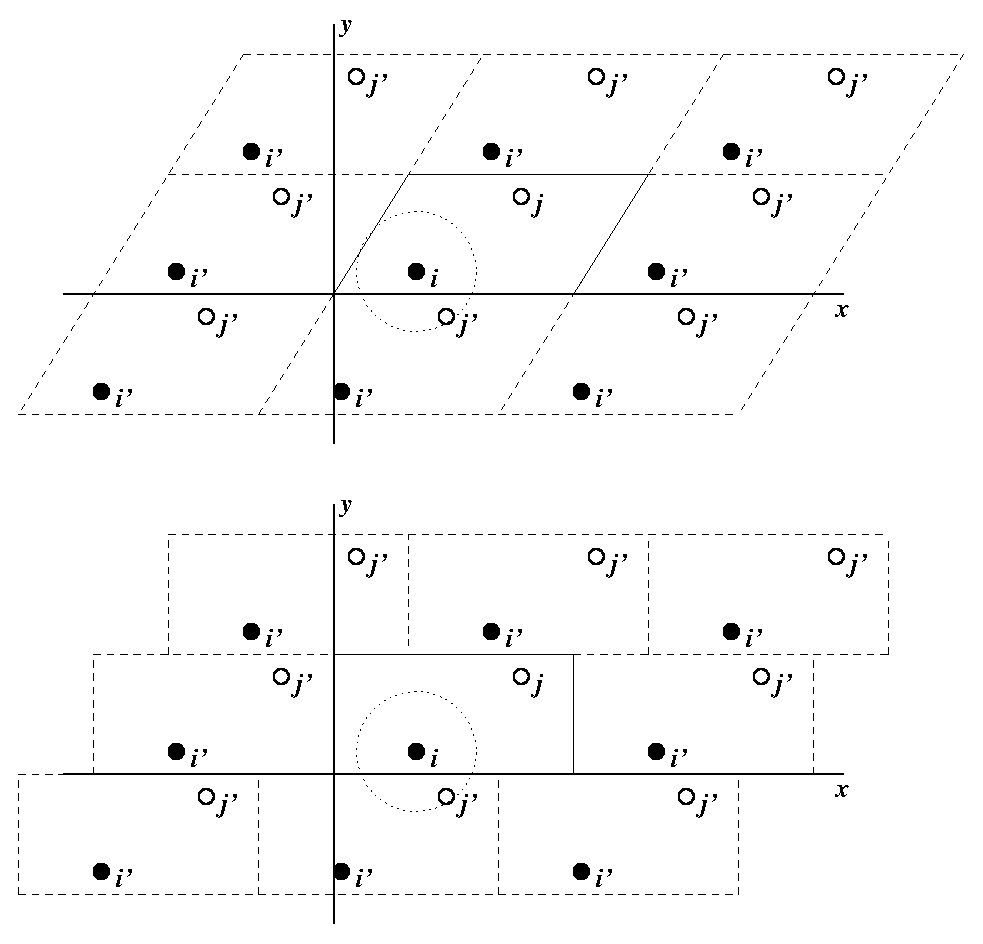
\includegraphics[width=9cm]{plots/pbctric}}
\caption {Periodic boundary conditions in two dimensions.}
\label{fig:pbc}
\end{figure}
The classical way to minimize edge effects in a finite system is to
apply {\em periodic boundary conditions}. The atoms of the system to
be simulated are put into a space-filling box, which is surrounded by
translated copies of itself (\figref{pbc}).  Thus there are no
boundaries of the system; the artifact caused by unwanted boundaries
in an isolated cluster is now replaced by the artifact of periodic
conditions. If a crystal is simulated, such boundary conditions are
desired (although motions are naturally restricted to periodic motions
with wavelengths fitting into the box). If one wishes to simulate
non-periodic systems, as liquids or solutions, the periodicity by
itself causes errors. The errors can be evaluated by comparing various
system sizes; they are expected to be less severe than the errors
resulting from an unnatural boundary with vacuum.

There are several possible shapes for space-filling unit cells. Some,
as the {\em rhombic dodecahedron} and the 
{\em truncated octahedron}~\cite{Adams79} are closer to a sphere
than a cube is and are therefore more economical for
studying an (approximately spherical) macromolecule in solution, since
fewer solvent molecules are required to fill the box given a minimum
distance between macromolecular images. However, a periodic system
based on the rhombic dodecahedron or truncated octahedron is equivalent
to a periodic system based on a {\em triclinic} unit cell.
The latter shape is the most general space-filling unit cell;
it comprises all possible space-filling shapes~\cite{Bekker95}.
Therefore {\gromacs} is based on the triclinic unit cell.
  
{\gromacs} uses periodic boundary conditions, combined with the {\em
minimum image convention:} only one - the nearest - image of each
particle is considered for short-range non-bonded interaction terms.
For long-range electrostatic interactions this is not always accurate
enough, and {\gromacs} therefore also incorporates lattice sum methods
like Ewald Sum, PME and PPPM.

Gromacs supports triclinic boxes of any shape.
The box is defined by the 3 box vectors ${\bf a}$,${\bf b}$ and ${\bf c}$.
The box vectors must satisfy the following conditions:
\beq
\label{eqn:box_rot}
a_y = a_z = b_z = 0
\eeq
\beq
\label{eqn:box_shift1}
a_x>0,~~~~b_y>0,~~~~c_z>0
\eeq
\beq
\label{eqn:box_shift2}
|b_x| \leq \frac{1}{2} \, a_x,~~~~
|c_x| \leq \frac{1}{2} \, a_x,~~~~
|c_y| \leq \frac{1}{2} \, b_y
\eeq
Equations \ref{eqn:box_rot} can always be statisfied by rotating the box.
Inequalities (\ref{eqn:box_shift1}) and (\ref{eqn:box_shift2}) can always be
statisfied by adding and subtracting box vectors.

Even when simulating using a triclinic box, {\gromacs} always puts the
particles in a brick shaped volume, for efficiency reasons.
This is illustrated in \figref{pbc} for a 2-dimensional system.
So from the output trajectory it might seem like the simulation was done in
a rectangular box. The program {\tt trjconv} can be used to convert the
trajectory to a different unit-cell representation.

It is also possible to simulate without periodic boundary conditions,
but it is more efficient to simulate an isolated cluster of molecules
in a large periodic box, since fast grid searching can only be used 
in a periodic system.

\begin{figure}
\centerline{
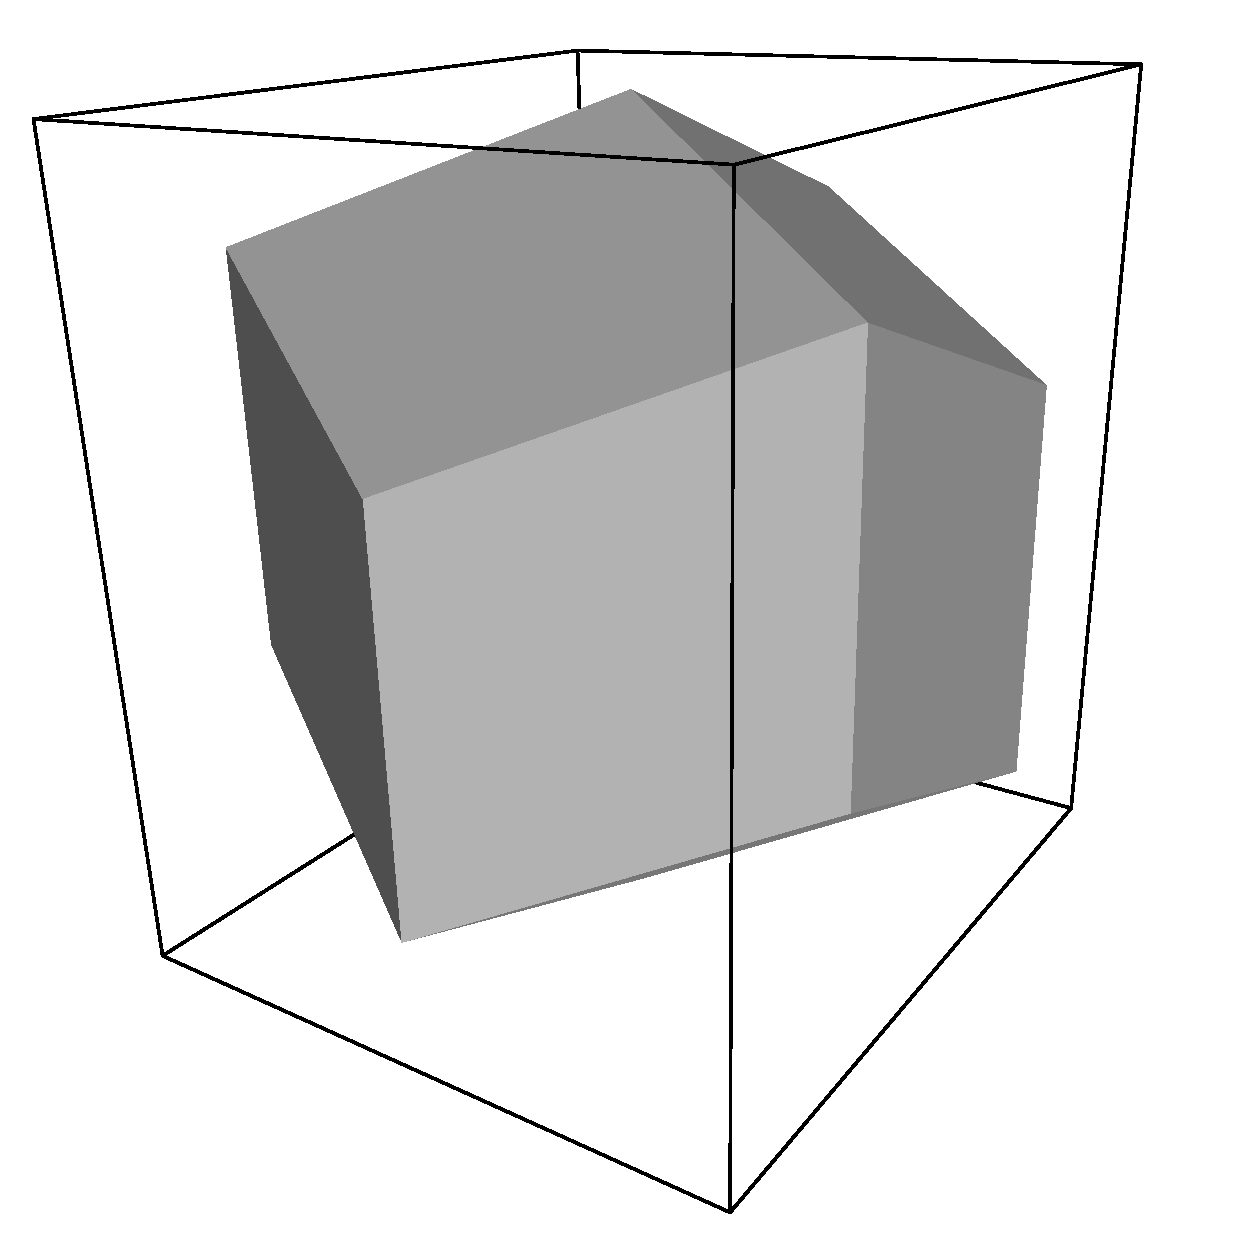
\includegraphics[width=5cm]{plots/rhododec}
~~~~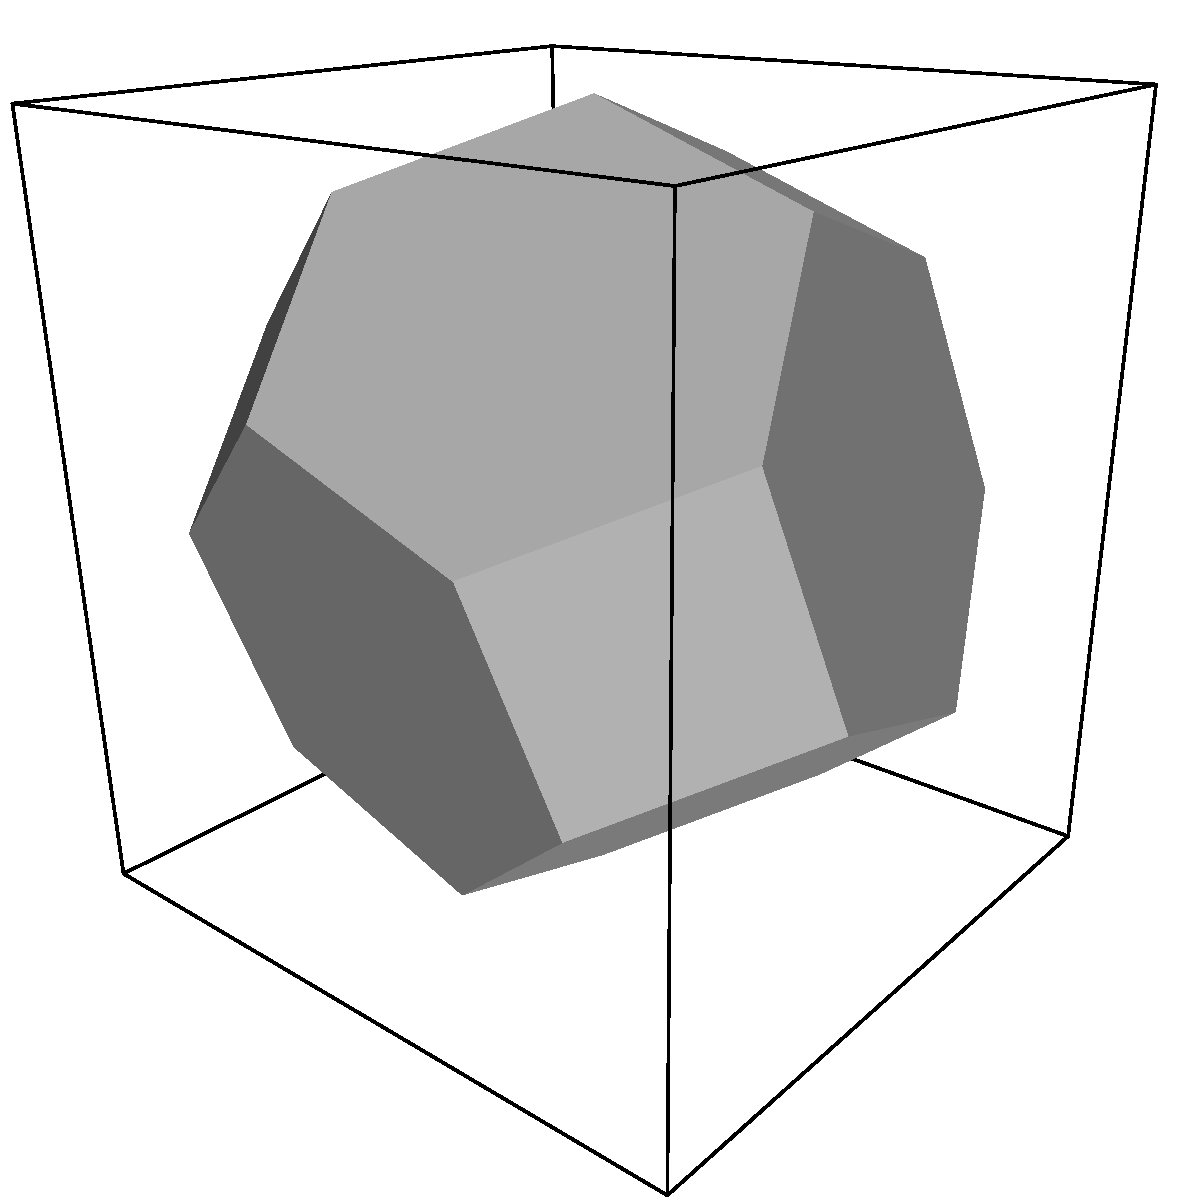
\includegraphics[width=5cm]{plots/truncoct}
}
\caption {A rhombic dodecahedron and truncated octahedron
(arbitrary orientations).}
\label{fig:boxshapes}
\end{figure}

\subsection{Some useful box types}
\begin{table}
\centerline{
\begin{tabular}{|c|c|c|ccc|ccc|}
\dline
box type & image & box & \multicolumn{3}{c|}{box vectors} & \multicolumn{3}{c|}{box vector angles} \\
 & distance & volume & ~{\bf a}~ & {\bf b} & {\bf c} &
   $\angle{\bf bc}$ & $\angle{\bf ac}$ & $\angle{\bf ab}$ \\
\dline
             &     &       & $d$ & 0              & 0              & & & \\
cubic        & $d$ & $d^3$ & 0   & $d$            & 0              & $90^\circ$ & $90^\circ$ & $90^\circ$ \\
             &     &       & 0   & 0              & $d$            & & & \\
\hline
rhombic      &     &       & $d$ & 0              & $\frac{1}{2}\,d$ & & & \\
dodecahedron & $d$ & $\frac{1}{2}\sqrt{2}\,d^3$ & 0   & $d$            & $\frac{1}{2}\,d$ & $60^\circ$ & $60^\circ$ & $90^\circ$ \\
(xy-square)  &     & $0.707\,d^3$ & 0   & 0              & $\frac{1}{2}\sqrt{2}\,d$ & & & \\
\hline
rhombic      &     &       & $d$ & $\frac{1}{2}\,d$ & $\frac{1}{2}\,d$ & & & \\
dodecahedron & $d$ & $\frac{1}{2}\sqrt{2}\,d^3$ & 0 & $\frac{1}{2}\sqrt{3}\,d$ & $\frac{1}{6}\sqrt{3}\,d$ & $60^\circ$ & $60^\circ$ & $60^\circ$ \\
(xy-hexagon) &     & $0.707\,d^3$ & 0   & 0              & $\frac{1}{3}\sqrt{6}\,d$ & & & \\
\hline
truncated    &     &       & $d$ & $\frac{1}{3}\,d$ & $-\frac{1}{3}\,d$ & & &\\
octahedron   & $d$ & $\frac{4}{9}\sqrt{3}\,d^3$ & 0   & $\frac{2}{3}\sqrt{2}\,d$ & $\frac{1}{3}\sqrt{2}\,d$ & $71.53^\circ$ & $109.47^\circ$ & $71.53^\circ$ \\
             &     & $0.770\,d^3$ & 0   & 0              & $\frac{1}{3}\sqrt{6}\,d$ & & & \\
\dline
\end{tabular}
}
\caption{The cubic box, the rhombic \normindex{dodecahedron} and the truncated
\normindex{octahedron}.}
\label{tab:boxtypes}
\end{table}
The three most useful box types for simulations of solvated systems
are described in \tabref{boxtypes}.  The rhombic dodecahedron
(\figref{boxshapes}) is the smallest and most regular space-filling
unit cell. Each of the 12 image cells is at the same distance.  The
volume is 71\% of the volume of a cube having the same image
distance. This saves about 29\% of CPU-time when simulating a
spherical or flexible molecule in solvent. There are two different
orientations of a rhombic dodecahedron that satisfy equations
\ref{eqn:box_rot}, \ref{eqn:box_shift1} and \ref{eqn:box_shift2}.
The program {\tt editconf} produces the orientation
which has a square intersection with the xy-plane.  This orientation
was chosen because the first two box vectors coincide with the x and
y-axis, which is easier to comprehend. The other orientation can be
useful for simulations of membrane proteins. In this case the
cross-section with the xy-plane is a hexagon, which has an area which
is 14\% smaller than the area of a square with the same image
distance.  The height of the box ($c_z$) should be changed to obtain
an optimal spacing.  This box shape not only saves CPU-time, it
also results in a more uniform arrangement of the proteins.

\subsection{Cutoff restrictions}
The minimum image convention implies that the cutoff radius used to
truncate non-bonded interactions must not exceed half the shortest box
vector:
\beq
\label{eqn:physicalrc}
  R_c < \half \min(\|{\bf a}\|,\|{\bf b}\|,\|{\bf c}\|),
\eeq
otherwise more than one image would be within the cutoff distance of
the force. When a macromolecule, such as a protein, is studied in
solution,  this restriction does not suffice. In principle a single
solvent  molecule should not be able
to `see' both sides of the macromolecule. This means that the length of
each box vector must exceed the length of the macromolecule in the
direction of that edge {\em plus} two times the cutoff radius $R_c$.
It is common to compromise in this respect, and make the solvent layer
somewhat smaller in order to reduce the computational cost.
For efficiency reasons the cutoff with triclinic boxes is more restricted.
For grid search the extra restriction is weak:
\beq
\label{eqn:gridrc}
R_c < \min(a_x,b_y,c_z)
\eeq
For simple search the extra restriction is stronger:
\beq
\label{eqn:simplerc}
R_c < \half \min(a_x,b_y,c_z)
\eeq

Each unit cell (cubic, rectangular or triclinic)
is surrounded by 26 translated images. Thus a
particular image can always be identified by an index pointing to one
of 27 {\em translation vectors} and constructed by applying a
translation with the indexed vector (see \ssecref{forces}).
Restriction (\ref{eqn:gridrc}) ensures that only 26 images need to be
considered.

%\ifthenelse{\equal{\gmxlite}{1}}{}{
\section{The group concept}
\label{sec:group}
In the {\gromacs} MD and analysis programs one uses {\em groups} of
atoms to perform certain actions on. The maximum number of groups is
256, but each atom can only belong to six different groups, one 
each of the following:
\begin{description}
\item[T-coupling group]
The \swapindex{temperature}{coupling} parameters (reference
temperature, time constant, number of degrees of freedom, see
\ssecref{update}) can be defined for each T-coupling group
separately. For example, in a solvated macromolecule the solvent (that
tends to generate more heating by force and integration errors) can be
coupled with a shorter time constant to a bath than is a macromolecule,
or a surface can be kept cooler than an adsorbing molecule. Many
different T-coupling groups may be defined. See also center of mass
groups below.

\item[\swapindex{Freeze}{group}]
Atoms that belong to a freeze group are kept stationary in the
dynamics. This is useful during equilibration, {\eg} to avoid badly
placed solvent molecules giving unreasonable kicks to protein atoms,
although the same effect can also be obtained by putting a restraining
potential on the atoms that must be protected. The freeze option can
be used, if desired, on just one or two coordinates of an atom,
thereby freezing the atoms in a plane or on a line.  When an atom is
partially frozen, constraints will still be able to move it, even in a
frozen direction. A fully frozen atom can not be moved by constraints.
Many freeze groups can be defined.  Frozen coordinates are unaffected
by pressure scaling, in some cases this can produce unwanted results,
in particular when constraints are used as well (in this case you will
get very large pressures).  Because of this it is recommended to not
combine freeze groups with constraints and pressure coupling. For the
sake of equilibration it could suffice to start with freezing in a
constant volume simulation, and afterwards use position restraints in
conjunction with constant pressure.

\item[Accelerate group]
On each atom in an '\swapindex{accelerate}{group}' an acceleration
$\ve{a}^g$ is imposed. This is equivalent to an external
force. This feature makes it possible to drive the system into a
non-equilibrium state and enables the performance of 
\swapindex{non-equilibrium}{MD} and hence to obtain transport properties.

\item[\swapindex{Energy monitor}{group}]
Mutual interactions between all energy monitor groups are compiled
during the simulation. This is done separately for Lennard-Jones and
Coulomb terms.  In principle up to 256 groups could be defined, but
that would lead to 256$\times$256 items! Better use this concept
sparingly.

All non-bonded interactions between pairs of energy monitor groups can
be excluded\index{exclusions, energy monitor group} (see \secref{mdpopt}).
Pairs of particles from excluded pairs of energy monitor groups
are not put into the pair list.
This can result in a significant speedup
for simulations where interactions within or between parts of the system
are not required.

\item[Center of mass group]
In \gromacs\ the center of mass (COM) motion can be removed, for
either the complete system or for groups of atoms. The latter is
useful, {\eg} for systems where there is limited friction ({\eg} gas
systems) to prevent center of mass motion to occur. It makes sense to
use the same groups for Temperature coupling and center of mass motion
removal.

\item[XTC output group]
In order to reduce the size of the \normindex{XTC} trajectory file, only a subset
of all particles can be stored. All XTC groups that are specified
are saved, the rest is not. If no XTC groups are specified, than all
atoms are saved to the XTC file.

\end{description}
The use of groups in analysis programs is described in
\chref{analysis}.
%} % Brace matches ifthenelse test for gmxlite

\section{Molecular Dynamics}
\label{sec:MD}
\begin{figure}
\begin{center}
\addtolength{\fboxsep}{0.5cm}
\begin{shadowenv}[12cm]
{\large \bf THE GLOBAL MD ALGORITHM}
\rule{\textwidth}{2pt} \\
{\bf 1. Input initial conditions}\\[2ex]
Potential interaction $V$ as a function of atom positions\\
Positions $\ve{r}$ of all atoms in the system\\
Velocities $\ve{v}$ of all atoms in the system \\
$\Downarrow$\\
\rule{\textwidth}{1pt}\\
{\bf repeat 2,3,4} for the required number of steps:\\
\rule{\textwidth}{1pt}\\
{\bf 2. Compute forces} \\[1ex]
The force on any atom  \\[1ex]
$\ve{F}_i = - \displaystyle\frac{\partial V}{\partial \ve{r}_i}$ \\[1ex]
is computed by calculating the force between non-bonded atom pairs: \\
$\ve{F}_i = \sum_j \ve{F}_{ij}$ \\
plus the forces due to bonded interactions (which may depend on 1, 2,
3, or 4 atoms), plus restraining and/or external forces. \\
The potential and kinetic energies and the pressure tensor are computed. \\   
$\Downarrow$\\
{\bf 3. Update configuration} \\[1ex]
The movement of the atoms is simulated by numerically solving Newton's
equations of motion \\[1ex]
$\displaystyle
\frac {\de^2\ve{r}_i}{\de t^2} = \frac{\ve{F}_i}{m_i} $ \\
or \\
$\displaystyle
\frac{\de\ve{r}_i}{\de t} = \ve{v}_i ; \;\;
\frac{\de\ve{v}_i}{\de t} = \frac{\ve{F}_i}{m_i} $ \\[1ex]
$\Downarrow$ \\
{\bf 4.} if required: {\bf Output step} \\
write positions, velocities, energies, temperature, pressure, etc. \\
\end{shadowenv}
\caption{The global MD algorithm}
\label{fig:global}
\end{center}
\end{figure}
A global flow scheme for MD is given in \figref{global}. Each
MD or  EM run requires as input a set of initial coordinates and -
optionally - initial velocities of all particles involved. This
chapter does not describe how these are obtained; for the setup of an
actual MD run check the online manual at {\wwwpage}.

\subsection{Initial conditions}
\subsubsection{Topology and force field}
The system topology, including a description of the force field, must
be loaded. These items are described in \chref{ff}.
All this information is static; it is never modified during the run.

\subsubsection{Coordinates and velocities}
\begin{figure}
\centerline{\includegraphics[width=8cm]{plots/maxwell}}
\caption{A Maxwellian velocity distribution, generated from random numbers.}
\label{fig:maxwell}
\end{figure}

Then, before a run starts, the box size and the coordinates and
velocities of  all particles are required. The box size is determined
by three vectors (nine numbers) $\ve{b}_1, \ve{b}_2, \ve{b}_3$, which
represent the three basis vectors of the periodic box. While in the
present version of {\gromacs} only rectangular boxes are allowed, three
numbers  suffice, but the use of three vectors already
prepares for arbitrary triclinic boxes to be implemented in a later
version. 

If the run starts at $t=t_0$, the coordinates at $t=t_0$ must be
known. The {\em leap-frog algorithm,} used to update the time step
with $\Dt$ (see \ssecref{update}), requires that the velocities at
$t=t_0 - \hDt$ are known. If velocities are not available, the program
can generate initial atomic velocities $v_i, i=1\ldots 3N$ with a
\swapindex{Maxwellian}{distribution} (\figref{maxwell}) at a given
absolute temperature $T$:
\beq 
p(v_i) = \sqrt{\frac{m_i}{2 \pi kT}}\exp(-\frac{m_i v_i^2}{2kT})
\eeq
where $k$ is Boltzmann's constant (see \chref{defunits}).
To accomplish this, normally distributed random numbers are generated
by adding twelve random numbers $R_k$ in the range $0 \le R_k < 1$ and
subtracting 6.0 from their sum. The result is then multiplied by the
standard deviation of the velocity distribution $\sqrt{kT/m_i}$. Since
the resulting total energy will not correspond exactly to the required
temperature $T$, a correction is made: first the center-of-mass motion
is removed and then all velocities are scaled so that the total
energy corresponds exactly to $T$ (see \eqnref{E-T}).

\subsubsection{Center-of-mass motion}
The \swapindex{center-of-mass}{velocity} is normally set to zero at
every step.  Normally there is no net external force acting on the
system and the center-of-mass velocity should remain constant. In
practice, however, the update algorithm develops a very slow change in
the center-of-mass velocity, and thus in the total kinetic energy of
the system, specially when temperature coupling is used. If such
changes are not quenched, an appreciable center-of-mass motion
develops eventually in long runs, and the temperature will be
significantly misinterpreted. The same may happen due to overall
rotational motion, but only when an isolated cluster is simulated. In
periodic systems with filled boxes, the overall rotational motion is
coupled to other degrees of freedom and does not give any problems.


\subsection{\swapindex{Neighbor}{searching}}
\label{subsec:ns}
As mentioned in \chref{ff}, internal forces are
either generated from fixed (static) lists, or from dynamics lists.
The latter concern non-bonded interactions between any pair of particles.
When calculating the non-bonded forces, it is convenient to have all
particles in a rectangular box.
As shown in \figref{pbc}, it is possible to transform a
triclinic box into a rectangular box.
The output coordinates are always in a rectangular box, even when a
dodecahedron or triclinic box was used for the simulation.
Equation \ref{eqn:box_rot} ensures that we can reset particles
in a rectangular box by first shifting them with
box vector ${\bf c}$, then with ${\bf b}$ and finally with ${\bf a}$.
Equations \ref{eqn:box_shift2}, \ref{eqn:physicalrc} and \ref{eqn:gridrc}
ensure that we can find the 14 nearest triclinic images within
a linear combination which does not involve multiples of box vectors.

\subsubsection{Pair lists generation}
The non-bonded pair forces need to be calculated only for those pairs
$i,j$  for which the distance $r_{ij}$ between $i$ and the 
\swapindex{nearest}{image} 
of $j$ is less than a given cutoff radius $R_c$. Some of the particle
pairs that fulfill this criterion are excluded, when their interaction
is already fully accounted for by bonded interactions.  {\gromacs}
employs a {\em pair list} that contains those particle pairs for which
non-bonded forces must be calculated.  The pair list contains atoms
$i$, a displacement vector for atom $i$, and all particles $j$ that
are within \verb'rshort' of this particular image of atom $i$.  The
list is updated every \verb'nstlist' steps, where \verb'nstlist' is
typically 10. There is an option to calculate the total non-bonded
force on each particle due to all particle in a shell around the
list-cutoff, {\ie} at a distance between \verb'rshort' and
\verb'rlong'.  This force is calculated during the pair list update
and  retained during \verb'nstlist' steps.

To make the \normindex{neighbor list} all particles that are close
({\ie} within the neighbor list cutoff) to a given particle must be found.
This searching, usually called neighbor searching (NS),
involves periodic boundary conditions and determining the {\em image}
(see \secref{pbc}). Without periodic boundary conditions a simple
$O(N^2)$ algorithm must be used. With periodic boundary conditions
a grid search can be used, which is $O(N)$.

\ifthenelse{\equal{\gmxlite}{1}}{}{
To completely avoid cut-off artifacts, the non-bonded potentials
can be switched exactly to zero at some distance smaller
than the neighbor list cut-off (there are several ways to do this
in {\gromacs}, see \secref{mod_nb_int}).
One then has a buffer with the size equal to the neighbor list
cut-off minus the longest interaction cut-off.
In this case one can also choose to let {\tt mdrun} only update
the neighbor list when required. That is when one or more particles
have moved more than half the buffer size from the center of geometry
of the charge group they belong to (see \secref{chargegroup})
as determined at the previous neighbor search.
This option guarantees that their are no cut-off artifacts.
Note that for larger systems this comes at a high computational cost,
since the neighbor list update frequency will be determined
by just one or two particles moving slightly beyond the half buffer length
(which not even necessarily implies that the neighbor list is invalid),
while 99.99\% of the particles are fine.
} % Brace matches ifthenelse test for gmxlite

\subsubsection{\swapindex{Simple}{search}}
Due to \eqnsref{box_rot}{simplerc}, the vector $\rvij$
connecting images within the cutoff $R_c$ can be found by constructing:
\begin{eqnarray}
\ve{r}'''   & = & \ve{r}_j-\ve{r}_i \\
\ve{r}''    & = & \ve{r}''' - {\bf c}*\verb'round'(r'''_z/c_z)) \\
\ve{r}'     & = & \ve{r}'' - {\bf b}*\verb'round'(r''_y/b_y) \\
\ve{r}_{ij} & = & \ve{r}' - {\bf a}*\verb'round'(r'_x/a_x)
\end{eqnarray}
When distances between two particles in a triclinic box are needed
that do not obey \eqnref{box_rot},
many shifts of combinations of box vectors need to be considered to find
the nearest image.

\ifthenelse{\equal{\gmxlite}{1}}{}{

\begin{figure}
\centerline{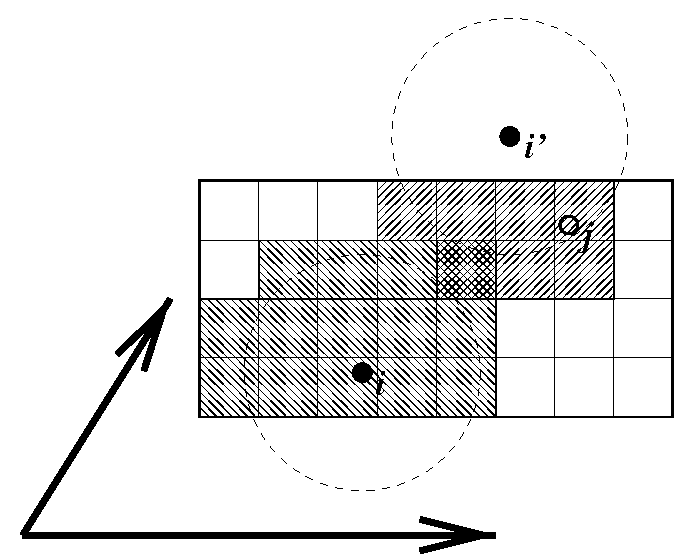
\includegraphics[width=8cm]{plots/nstric}}
\caption {Grid search in two dimensions. The arrows are the box vectors.}
\label{fig:grid}
\end{figure}

\subsubsection{\swapindex{Grid}{search}}
\label{sec:nsgrid}
The grid search is schematically depicted in \figref{grid}.  All
particles are put on the {\nsgrid}, with the smallest spacing $\ge$
$R_c/2$ in each of the directions.  In the direction of each box
vector, a particle $i$ has three images. For each direction the image
may be -1,0 or 1, corresponding to a translation over -1, 0 or +1 box
vector. We do not search the surrounding {\nsgrid} cells for neighbors
of $i$ and then calculate the image, but rather construct the images
first and then search neighbors corresponding to that image of $i$.
As \figref{grid} shows, some grid cells may be searched more than once
for different images of $i$. This is not a problem, since, due to the
minimum image convention, at most one image will ``see'' the
$j$-particle.  For every particle, fewer than 125 (5$^3$) neighboring
cells are searched.  Therefore, the algorithm scales linearly with the
number of particles.  Although the prefactor is large, the scaling
behavior makes the algorithm far superior over the standard $O(N^2)$
algorithm when there are more than a few hundred particles.  The
grid search is equally fast for rectangular and triclinic boxes.  Thus
for most protein and peptide simulations the rhombic dodecahedron will
be the preferred box shape.
} % Brace matches ifthenelse test for gmxlite

\ifthenelse{\equal{\gmxlite}{1}}{}{
\subsubsection{Charge groups}
\label{sec:chargegroup}
Where applicable, neighbor searching is carried out on the basis of
{\em charge groups}. A \swapindex{charge}{group} is a small set of
nearby atoms with an integer net charge. Charge groups are defined in
the molecular topology. If the nearest image distance between the {\em
geometrical centers} of the atoms of two charge groups is less than
the cutoff radius, all atom pairs between the charge groups are
included in the pair list. This procedure avoids the creation of
charges due to the use of a cutoff (when one charge of a dipole is
within range and the other not), which can have disastrous
consequences for the behavior of the Coulomb interaction function at
distances near the cutoff radius. If molecular groups have full
charges (ions), charge groups do not avoid adverse cutoff effects,
and you should consider using one of the lattice sum methods supplied
by {\gromacs}~\cite{Berendsen93a}.

If appropriately
constructed \swapindex{shift}{function}s are used for the 
\swapindex{electrostatic}{force}s, no
charge groups are needed. Such shift functions are implemented in
{\gromacs} (see \chref{ff}) but must be used with care: in principle,
they should be combined with a lattice sum for long-range
electrostatics.

Charge groups also provide a speed up of the neighbor search.
The neighbor searching for a water system, for instance,
is $3^2=9$ times faster when each molecule is treated as a charge group.
Also the highly optimized water force loops (see \secref{waterloops})
only work when all atoms in a water molecule form a single charge group.
} % Brace matches ifthenelse test for gmxlite

\subsection{Compute forces}
\label{subsec:forces}

\subsubsection{Potential energy}
When forces are computed, the \swapindex{potential}{energy} of each
interaction term is computed as well. The total potential energy is
summed for various contributions, such as Lennard-Jones, Coulomb, and
bonded terms. It is also possible to compute these contributions for
{\em groups} of atoms that are separately defined (see
\secref{group}).

\subsubsection{Kinetic energy and temperature}
The \normindex{temperature} is given by the total
\swapindex{kinetic}{energy} of the $N$-particle system:
\beq
E_{kin} = \half \sum_{i=1}^N m_i v_i^2
\eeq
From this the absolute temperature $T$ can be computed using:
\beq
\half N_{df} kT = E_{kin}
\label{eqn:E-T}
\eeq
where $k$ is Boltzmann's constant and $N_{df}$ is the number of
degrees of freedom which can be computed from:
\beq
N_{df}  ~=~     3 N - N_c - N_{com}
\eeq
Here $N_c$ is the number of {\em constraints} imposed on the system.
When performing molecular dynamics $N_{com}=3$ additional degrees of
freedom must be removed, because the three
center-of-mass velocities are constants of the motion, which are usually
set to zero. When simulating in vacuo, the rotation around the center of mass
can also be removed, in this case $N_{com}=6$.
When more than one temperature coupling group is used, the number of degrees
of freedom for group $i$ is:
\beq
N^i_{df}  ~=~  (3 N^i - N^i_c) \frac{3 N - N_c - N_{com}}{3 N - N_c}
\eeq

The kinetic energy can also be written as a tensor, which is necessary
for pressure calculation in a triclinic system, or systems where shear
forces  are imposed:
\beq
{\bf E}_{kin} = \half \sum_i^N m_i \vvi \otimes \vvi
\eeq

\subsubsection{Pressure and virial}
The \normindex{pressure} 
tensor {\bf P} is calculated from the difference between 
kinetic energy $E_{kin}$ and the \normindex{virial} ${\bf \Xi}$
\beq
{\bf P} = \frac{2}{V} ({\bf E}_{kin}-{\bf \Xi})
\label{eqn:P}
\eeq
where $V$ is the volume of the computational box. 
The scalar pressure $P$, which can be used for pressure coupling in the case
of isotropic systems, is computed as:
\beq
P       = {\rm trace}({\bf P})/3
\eeq

The virial ${\bf \Xi}$ tensor is defined as 
\beq
{\bf \Xi} = -\half \sum_{i<j} \rvij \otimes \Fvij 
\label{eqn:Xi}
\eeq

\ifthenelse{\equal{\gmxlite}{1}}{}{
The {\gromacs} implementation of the virial computation is described
in \secref{virial}.
} % Brace matches ifthenelse test for gmxlite


\subsection{Update configuration}
\label{subsec:update}
\begin{figure}
\centerline{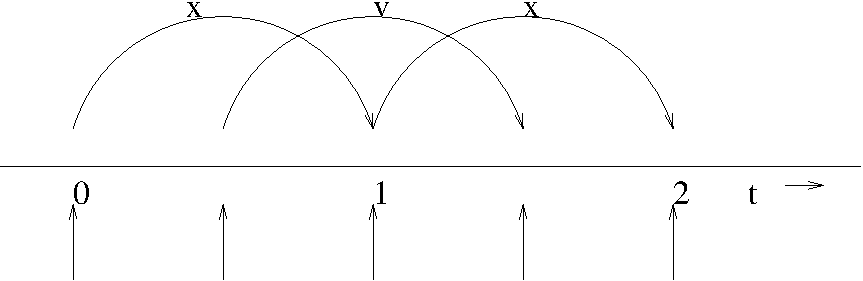
\includegraphics[width=8cm]{plots/leapfrog}}
\caption[The Leap-Frog integration method.]{The Leap-Frog integration method. The algorithm is called Leap-Frog because r and v are leaping
like  frogs over each others back.}
\label{fig:leapfrog}
\end{figure}

The {\gromacs} MD program utilizes the so-called {\em leap-frog} 
algorithm~\cite{Hockney74} for the integration of the equations of
motion.  The \normindex{leap-frog} 
algorithm uses positions $\ve{r}$ at time $t$ and
velocities $\ve{v}$ at time $t-\hDt$; it updates positions and
velocities using the forces
$\ve{F}(t)$ determined by the positions at time $t$: 
\bea
\ve{v}(t+\hDt)  &~=~&   \ve{v}(t-\hDt)+\frac{\ve{F}(t)}{m}\Dt   \\
\ve{r}(t+\Dt)   &~=~&   \ve{r}(t)+\ve{v}(t+\hDt)\Dt
\eea
The algorithm is visualized in \figref{leapfrog}.
It is equivalent to the Verlet~\cite{Verlet67} algorithm:
\beq
\ve{r}(t+\Dt)~=~2\ve{r}(t) - \ve{r}(t-\Dt) + \frac{\ve{F}(t)}{m}\Dt^2+O(\Dt^4)
\eeq
The algorithm is of third order in $\ve{r}$ and is time-reversible.
See ref.~\cite{Berendsen86b} for the merits of this algorithm and comparison
with other time integration algorithms.
 
The \swapindex{equations of}{motion} are modified for temperature coupling
 and pressure coupling, and extended to include the conservation of
constraints, all of which are described below.

\subsection{\swapindex{Temperature}{coupling}}
\index{temperature coupling}
For several reasons (drift during equilibration, drift as a result of
force truncation and integration errors, heating due to external or
frictional forces), it is necessary to control the temperature of the
system. {\gromacs} can use either
the {\em weak coupling} scheme of Berendsen~\cite{Berendsen84} or
the extended ensemble Nos{\'e}-Hoover scheme~\cite{Nose84,Hoover85}.

\subsubsection{\swapindex{Berendsen}{temperature coupling}}
\index{weak coupling}
The Berendsen algorithm mimics weak coupling with first-order 
kinetics to an external heat bath with given temperature $T_0$. 
See ref.~\cite{Berendsen91} for a comparison with the
Nos{\'e}-Hoover scheme. The effect of this algorithm is
that a deviation of the system temperature from $T_0$ is slowly
corrected according to
\beq
\frac{\de T}{\de t} = \frac{T_0-T}{\tau}
\label{eqn:Tcoupling}
\eeq
which means that a temperature deviation decays exponentially with a
time constant $\tau$.
This method of coupling has the advantage that the strength of the
coupling can be varied and adapted to the user requirement: for
equilibration purposes the coupling time can be taken quite short
({\eg} 0.01 ps), but for reliable equilibrium runs it can be taken much
longer ({\eg} 0.5 ps) in which case it hardly influences the
conservative dynamics. 
 
The heat flow into or out of the system is effected by scaling the
velocities of each particle every step with a time-dependent factor
$\lambda$, given by
\beq 
\lambda = \left[ 1 + \frac{\Delta t}{\tau_T}
\left\{\frac{T_0}{T(t -  \hDt)} - 1 \right\} \right]^{1/2}
\label{eqn:lambda}
\eeq
The parameter $\tau_T$ is close to, but not exactly equal to the time constant
$\tau$ of the temperature coupling (\eqnref{Tcoupling}):
\beq
\tau = 2 C_V \tau_T / N_{df} k
\eeq
where $C_V$ is the total heat capacity of the system, $k$ is Boltzmann's
constant, and $N_{df}$ is the total number of degrees of freedom. The
reason that $\tau \neq \tau_T$ is that the kinetic energy change
caused by scaling the velocities is partly redistributed between
kinetic and potential energy and hence the change in temperature is
less than the scaling energy.  In practice, the ratio $\tau / \tau_T$
ranges from 1 (gas) to 2 (harmonic solid) to 3 (water). When we use
the term 'temperature coupling time constant', we mean the parameter
\normindex{$\tau_T$}.  
{\bf Note} that in practice the scaling factor $\lambda$ is limited to 
the range of 0.8 $<= \lambda <=$ 1.25, to avoid scaling by very large
numbers which may crash the simulation. In normal use, 
$\lambda$ will always be much closer to 1.0.
  
Strictly, for computing the scaling factor the temperature $T$ is
needed at time $t$, but this is not available in the algorithm. In
practice, the temperature at the previous time step is used (as
indicated in \eqnref{lambda}), which is perfectly all right since the
coupling time constant is much longer than one time step. The
Berendsen algorithm is stable up to $\tau_T \approx \Dt$.  [A simple
steepest-descent minimizer can be implemented by setting $T=0$ and
$\tau_T \ll \delta t$.]

\ifthenelse{\equal{\gmxlite}{1}}{}{
\subsubsection{\swapindex{Nos{\'e}-Hoover}{temperature coupling}}
\index{extended ensemble}
The Berendsen weak coupling algorithm is extremely efficient for relaxing
a system to the target temperature, but once your system
has reached equilibrium it might be more important to probe a
correct canonical ensemble. This is unfortunately not the case for
the weak coupling scheme, although the difference is usually negligible.

To enable canonical ensemble simulations, {\gromacs} also supports the 
extended-ensemble approach first proposed by Nos\'e\cite{Nose84} and later 
modified by Hoover\cite{Hoover85}. The system Hamiltonian 
is extended by introducing a 
thermal reservoir and a friction term in the equations of motion.
The friction force is proportional to the product of each particle's
velocity and a friction parameter $\xi$. This friction
parameter (or 'heat bath' variable) is a fully dynamic quantity with
its own equation of motion; the time 
derivative is calculated from the difference between the current
kinetic energy and the reference temperature. 

In Hoover's formulation, the particles' equations of motion in
\figref{global} are replaced by

\beq
\frac {\de^2\ve{r}_i}{\de t^2} = \frac{\ve{F}_i}{m_i} - 
\xi \frac{\de \ve{r}_i}{\de t} ,
\label{eqn:NH-eqn-of-motion}
\eeq

where the equation of motion for the heat bath parameter $\xi$ is

\beq
\frac {\de \xi}{\de t} = \frac{1}{Q}\left( T - T_0 \right).
\eeq

The reference temperature is denoted $T_0$, while $T$ is the current
instantaneous temperature of the system. The strength of the coupling is
determined by the constant $Q$ (usually called the 'mass parameter' 
of the reservoir) in combination with the reference temperature.

In our opinion, the mass parameter is a somewhat awkward way of 
describing coupling strength, especially due to its dependence on
reference temperature (and some implementations even include the number
of degrees of freedom in your system when defining $Q$). 
To maintain the coupling strength, one would have to change $Q$ in
proportion to the change in reference temperature. For this reason,
we prefer to let the {\gromacs} user work instead with the
period $\tau_T$ of the oscillations of kinetic energy between the 
system and the reservoir instead. It is directly related to $Q$ and $T_0$ via

\beq
Q = \frac {\tau_T^2 T_0}{4 \pi^2}.
\eeq

This provides a much more intuitive way of selecting the Nos{\'e}-Hoover
coupling strength (similar to the weak coupling relaxation), 
and in addition $\tau_T$ is independent of system size and reference
temperature. 

It is however important to keep the difference between the 
weak coupling scheme and the Nos\'e-Hoover algorithm in mind: 
Using weak coupling you get a
strongly damped {\em exponential relaxation}, 
while the Nos\'e-Hoover approach
produces an {\em oscillatory relaxation}. 
The actual time it takes to relax with Nos\'e-Hoover coupling is 
several times larger than the period of the
oscillations that you select. These oscillations (in contrast
to exponential relaxation) also means that
the time constant normally should be 4--5 times larger
than the relaxation time used with weak coupling, but your 
mileage may vary.
}  % Brace matches ifthenelse test for gmxlite

\subsubsection{\swapindex{Group}{temperature coupling}}
In {\gromacs} temperature coupling can be performed on groups of
atoms, typically a protein and solvent. The reason such algorithmes
were introduced is that energy exchange between different components
is not perfect, due to different effects including cutoffs etc. If
now the whole system is coupled to one heat bath, water (which
experiences the largest cutoff noise) will tend to heat up and the
protein will cool down. Typically 100 K differences can be obtained.
With the use of proper electrostatic methods (PME) these difference
are much smaller but still not negligable. The parameters for
temperature coupling in groups are given in the {\tt mdp} file. One
special case should be mentioned: it is possible to T-couple only part
of the system (or nothing at all obviously). This is done by
specifying zero for the time constant $\tau_T$ for the group of interest.


\subsection{\swapindex{Pressure}{coupling}}
In the same spirit as the temperature coupling, the system can also be
coupled to a 'pressure bath'. 
{\gromacs} supports both the Berendsen algorithm~\cite{Berendsen84} 
that scales coordinates and box vectors every step, and the 
extended ensemble Parrinello-Rahman approach. Both of these can be
combined with any of the temperature coupling methods above.

\subsubsection{Berendsen pressure coupling}
\label{sec:berendsen_pressure_coupling}
\index{weak coupling}
The Berendsen algorithm rescales the 
coordinates and box vectors every step with a matrix {\boldmath $\mu$},
which has the effect of a first-order kinetic relaxation of the pressure
towards a given reference pressure ${\bf P}_0$:
\beq
\frac{\de {\bf P}}{\de t} = \frac{{\bf P}_0-{\bf P}}{\tau_p}
\eeq
The scaling matrix {\boldmath $\mu$} is given by
\beq
\mu_{ij}
= \delta_{ij} - \frac{\Delta t}{3\, \tau_p} \beta_{ij} \{P_{0ij} - P_{ij}(t) \}
\label{eqn:mu}
\eeq
\index{isothermal compressibility}
\index{compressibility}
Here {\boldmath $\beta$} is the isothermal compressibility of the system.
In most cases this will be a diagonal matrix, with equal elements on the
diagonal, the value of which is generally not known.
It suffices to take a rough estimate because the value of {\boldmath $\beta$}
only influences the non-critical time constant of the
pressure relaxation without affecting the average pressure itself.
For water at 1 atm and 300 K 
$\beta = 4.6 \times 10^{-10}$ Pa$^{-1} = 4.6 \times 10^{-5}$ Bar$^{-1}$,
which is $7.6 \times 10^{-4}$ MD units (see \chref{defunits}).
Most other liquids have similar values.
When scaling completely anisotropically, the system has to be rotated in
order to obey \eqnref{box_rot}.
This rotation is approximated in first order in the scaling, which is usually
less than $10^{-4}$. The actual scaling matrix {\boldmath $\mu'$} is:
\beq
\mbox{\boldmath $\mu'$} = 
\left(\begin{array}{ccc}
\mu_{xx} & \mu_{xy} + \mu_{yx} & \mu_{xz} + \mu_{zx} \\
0        & \mu_{yy}            & \mu_{yz} + \mu_{zy} \\
0        & 0                   & \mu_{zz}
\end{array}\right)                             
\eeq
The velocities are neither scaled nor rotated.

In {\gromacs}, the Berendsen scaling can also be done isotropically, 
which means that instead of $\ve{P}$ a diagonal matrix with elements of size
trace$(\ve{P})/3$ is used. For systems with interfaces, semi-isotropic 
scaling can be useful.
In this case the $x/y$-directions are scaled isotropically and the $z$
direction is scaled independently. The compressibility in the $x/y$ or
$z$-direction can be set to zero, to scale only in the other direction(s).

If you allow full anisotropic deformations and use constraints
you might have to scale more slowly or decrease your timestep to avoid 
errors from the constraint algorithms. 


\ifthenelse{\equal{\gmxlite}{1}}{}{
\subsubsection{\swapindex{Parrinello-Rahman}{pressure coupling}}

In cases where the fluctuations in pressure or volume 
are important {\em per se} ({\eg} to calculate thermodynamic
properties) it might at least theoretically be a problem that the 
exact ensemble is not well-defined for the weak coupling scheme. 

For this reason, {\gromacs} also supports constant-pressure simulations using 
the Parrinello-Rahman approach\cite{Parrinello81,Nose83}, which is similar
to the Nos\'e-Hoover temperature coupling. With the Parrinello-Rahman 
barostat, the box vectors as represented by the matrix \ve{b} obey
the matrix equation of motion\footnote{The box matrix representation \ve{b} in 
{\gromacs} corresponds to the transpose of the box matrix representation 
\ve{h} in the paper by Nos\'e and Klein. Because of this, some of our 
equations will look slightly different.}

\beq
\frac{\de \ve{b}^2}{\de t^2}= V \ve{W}^{-1} \ve{b}'^{-1} \left( \ve{P} - \ve{P}_{ref}\right).
\eeq

The volume of the box is denoted $V$, and $\ve{W}$ is a matrix parameter that determines
the strength of the coupling. The matrices \ve{P} and \ve{P}$_{ref}$ are the 
current and reference pressures, respectively.

The equations of motion for the particles are also changed, just as
for the Nos\'e-Hoover coupling. In most cases you would combine the 
Parrinello-Rahman barostat with the Nos\'e-Hoover
thermostat, but to keep it simple we only show the Parrinello-Rahman 
modification here:

\bea
\frac {\de^2\ve{r}_i}{\de t^2} & = & \frac{\ve{F}_i}{m_i} - 
\ve{M} \frac{\de \ve{r}_i}{\de t} , \\
\ve{M} & = & \ve{b}^{-1} \left[ \ve{b} \frac{\de \ve{b}'}{\de t} + \frac{\de \ve{b}}{\de t} \ve{b}' \right] \ve{b}'^{-1}.
\eea
The (inverse) mass parameter matrix $\ve{W}^{-1}$ determines the
strength of the coupling, and how the box can be deformed.
The box restriction (\ref{eqn:box_rot}) will be fulfilled automatically
if the corresponding elements of $\ve{W}^{-1}$ are zero. Since the
coupling strength also depends on the size of your box, we prefer
to calculate it automatically in {\gromacs}. 
You only have to provide the approximate
isothermal compressibilities {\boldmath $\beta$} 
and the pressure time constant $\tau_p$ in the input file
($L$ is the largest box matrix element):

\beq
\left( \ve{W}^{-1} \right)_{ij} = \frac{4 \pi^2 \beta_{ij}}{3 \tau_p^2 L}.
\eeq

Just as for the Nos\'e-Hoover thermostat, you should realize that
the Parrinello-Rahman time constant is {\em not} equivalent to the 
relaxation time used in the Berendsen pressure coupling algorithm. 
In most cases you will need to use a 4--5
times larger time constant with Parrinello-Rahman coupling. If
your pressure is very far from equilibrium, the Parrinello-Rahman
coupling may result in very
large box oscillations that could even crash your run. 
In that case you would have to increase the time constant, or (better)
use the weak coupling scheme to reach the target pressure, and then
switch to Parrinello-Rahman coupling once the system is in equilibrium.


\subsubsection{\swapindex{Surface tension}{coupling}}
When a periodic system consists of more than one phase, separated by
surfaces which are parallel to the xy-plane,
the surface tension and the z-component of the pressure can be coupled
to a pressure bath. Presently, this only works with the Berendsen
pressure coupling algorithm in {\gromacs}.
The average surface tension $\gamma(t)$ can be calculated from
the difference between the normal and the lateral pressure:
\begin{eqnarray}
\gamma(t) & = & 
\frac{1}{n} \int_0^{L_z}
\left\{ P_{zz}(z,t) - \frac{P_{xx}(z,t) + P_{yy}(z,t)}{2} \right\} \mbox{d}z \\
& = &
\frac{L_z}{n} \left\{ P_{zz}(t) - \frac{P_{xx}(t) + P_{yy}(t)}{2} \right\}
\end{eqnarray}
where $L_z$ is the height of the box and $n$ is the number of surfaces.
The pressure in the z-direction is corrected by scaling the height of
the box with $\mu_z$:
\beq
\Delta P_{zz} = \frac{\Delta t}{\tau_p} \{ P_{0zz} - P_{zz}(t) \}
\eeq
\beq
\mu_{zz} = 1 + \beta_{zz} \Delta P_{zz}
\eeq
This is similar to normal pressure coupling, except that the power
of one third is missing. 
The pressure correction in the z-direction is then used to get the
correct convergence for the surface tension to the reference value $\gamma_0$.
The correction factor for the box-length in the x/y-direction is:
\beq
\mu_{x/y} = 1 + \frac{\Delta t}{2\,\tau_p} \beta_{x/y}
        \left( \frac{n \gamma_0}{\mu_{zz} L_z}
        - \left\{ P_{zz}(t)+\Delta P_{zz} - \frac{P_{xx}(t) + P_{yy}(t)}{2} \right\} 
        \right)
\eeq
The value of $\beta_{zz}$ is more critical than with normal pressure
coupling. Normally an incorrect compressibility will just scale $\tau_p$,
but with surface tension coupling it affects the convergence of the surface
tension. 
When $\beta_{zz}$ is set to zero (constant box height), $\Delta P_z$ is also set
to zero, which is necessary for obtaining the correct surface tension. 
} % Brace matches ifthenelse test for gmxlite

\subsubsection{The complete update algorithm}
\begin{figure}
\begin{center}
\addtolength{\fboxsep}{0.5cm}
\begin{shadowenv}[12cm]
{\large \bf THE UPDATE ALGORITHM}
\rule{\textwidth}{2pt} \\
Given:\\
Positions $\ve{r}$ of all atoms at time $t$ \\
Velocities $\ve{v}$ of all atoms at time $t-\hDt$ \\
Accelerations $\ve{F}/m$ on all atoms at time $t$.\\
(Forces are computed disregarding any constraints)\\
Total kinetic energy and virial \\
$\Downarrow$ \\
{\bf 1.} Compute the scaling factors $\lambda$ and $\mu$\\
according to \eqnsref{lambda}{mu}\\   
$\Downarrow$ \\
{\bf 2.} Update and scale velocities: $\ve{v}' =  \lambda (\ve{v} +
\ve{a} \Delta t)$ \\
$\Downarrow$ \\
{\bf 3.} Compute new unconstrained coordinates: $\ve{r}' = \ve{r} + \ve{v}'
\Delta t$ \\
$\Downarrow$ \\
{\bf 4.} Apply constraint algorithm to coordinates: constrain($\ve{r}^{'} \rightarrow  \ve{r}'';
\,  \ve{r}$) \\
$\Downarrow$ \\
{\bf 5.} Correct velocities for constraints: $\ve{v} = (\ve{r}'' -
\ve{r}) / \Delta t$ \\
$\Downarrow$ \\
{\bf 6.} Scale coordinates and box: $\ve{r} = \mu \ve{r}''; \ve{b} =
\mu  \ve{b}$ \\
\end{shadowenv}
\caption{The MD update algorithm}
\label{fig:complete-update}
\end{center}
\end{figure}
The complete algorithm for the update of velocities and coordinates is
given in \figref{complete-update}. The SHAKE algorithm of step
4 is explained below. 

{\gromacs} has a provision to ''freeze''  (prevent motion of) selected
particles, which must be defined as a 'freeze group'. This is implemented
using a {\em freeze factor $\ve{f}_g$}, which is a vector, and differs for each
{\em freezegroup} (see \secref{group}). This vector contains only
zero (freeze) or one (don't freeze).
When we take this freeze factor and the external acceleration $\ve{a}_h$ into 
account the update algorithm for the velocities becomes:
\beq
\ve{v}(t+\hdt)~=~\ve{f}_g * \lambda * \left[ \ve{v}(t-\hdt) +\frac{\ve{F}(t)}{m}\Delta t + \ve{a}_h \Delta t \right]
\eeq
where $g$ and $h$ are group indices which differ per atom.

\subsection{Output step}
The important output of the MD run is the {\em
\swapindex{trajectory}{file}} \verb'name.trj' which contains particle coordinates
and -optionally- velocities at regular intervals. Since the trajectory
files are lengthy, one should not save every step! To retain all
information it suffices to write a frame every 15 steps, since at
least 30 steps are made per period of the highest frequency in the
system, and Shannon's \normindex{sampling} theorem states that two samples per
period of the highest frequency in a band-limited signal contain all
available information. But that still gives very long files! So, if
the highest frequencies are not of interest, 10 or 20 samples per ps
may suffice. Be aware of the distortion of high-frequency motions by
the {\em stroboscopic effect}, called {\em aliasing}: higher frequencies
are  mirrored with respect to the sampling frequency and appear as
lower frequencies. 

\ifthenelse{\equal{\gmxlite}{1}}{}{
\section{Shell molecular dynamics}
{\gromacs} can simulate \normindex{polarizability} using the 
\normindex{shell model} of Dick and Overhauser~\cite{Dick58}. In such models
a shell particle representing the electronic degrees of freedom is
attached to a nucleus by a spring. The potential energy is minimized with
respect to the shell position  at every step of the simulation (see below).
Succesfull applications of shell models in {\gromacs} have been published
for $N_2$~\cite{Jordan95} and water~\cite{Maaren2001a}.

\subsection{Optimization of the shell positions}
The force \ve{F}$_S$ on a shell particle $S$ can be decomposed into two
components:
\begin{equation}
\ve{F}_S ~=~ \ve{F}_{bond} + \ve{F}_{nb}
\end{equation}
where \ve{F}$_{bond}$ denotes the component representing the
polarization energy, usually represented by a harmonic potential and
\ve{F}$_{nb}$ is the sum of Coulomb and Van der Waals interactions. If we
assume that \ve{F}$_{nb}$ is almost constant we can analytically derive the
optimal position of the shell, i.e. where \ve{F}$_S$ = 0. If we have the
shell S connected to atom A we have
\begin{equation}
\ve{F}_{bond} ~=~ k_b \left( \ve{x}_S - \ve{x}_A\right)
\end{equation}
In an iterative solver, we have positions \ve{x}$_S(n)$ where $n$ is
the iteration count. We now have it iteration $n$:
\begin{equation}
\ve{F}_{nb} ~=~ \ve{F}_S - k_b \left( \ve{x}_S(n) - \ve{x}_A\right)
\end{equation}
and the optimal position for the shells $x_S(n+1)$ thus follows from
\begin{equation}
\ve{F}_S - k_b \left( \ve{x}_S(n) - \ve{x}_A\right) + k_b \left( \ve{x}_S(n+1) - \ve{x}_A\right) = 0
\end{equation}
if we write
\begin{equation}
\Delta \ve{x}_S = \ve{x}_S(n+1) - \ve{x}_S(n)
\end{equation}
we finally obtain
\begin{equation}
\Delta \ve{x}_S = \ve{F}_S/k_b
\end{equation}
which then yields the algorithm to compute the next trial in the optimization
of shell positions:
\begin{equation}
\ve{x}_S(n+1) ~=~ \ve{x}_S(n) + \ve{F}_S/k_b
\end{equation}
} % Brace matches ifthenelse test for gmxlite

\section{\normindex{Constraint} algorithms}
Constraints can be imposed in {\gromacs} using LINCS (default) or
the traditional SHAKE method.

\subsection{\normindex{SHAKE}}
The SHAKE~\cite{Ryckaert77} algorithm changes a set of unconstrained
coordinates $\ve{r}^{'}$ to a set of coordinates $\ve{r}''$ that
fulfill a  list of distance constraints, using a set $\ve{r}$ as
reference: \\[1ex] 
\hspace*{5em} SHAKE($\ve{r}^{'} \rightarrow  \ve{r}'';\,  \ve{r}$) \\[1ex]
This action is consistent with solving a set of Lagrange multipliers
in the constrained equations of motion. SHAKE needs a {\em tolerance}
\verb'TOL'; it will continue until all constraints are satisfied
within a {\em relative} tolerance \verb'TOL'. An error message is
given if SHAKE cannot reset the coordinates because the deviation is
too large, or if a given number of iterations is surpassed. 

Assume the equations of motion must fulfill $K$ holonomic constraints,
expressed as
\beq
\sigma_k(\ve{r}_1 \ldots \ve{r}_N) = 0; \;\; k=1 \ldots K
\eeq
({\eg} $(\ve{r}_1 - \ve{r}_2)^2 - b^2 = 0$). 
Then the forces are defined as 
\beq
- \frac{\partial}{\partial \ve{r}_i} \left( V + \sum_{k=1}^K \lambda_k
\sigma_k \right)
\eeq
where $\lambda_k$ are Lagrange multipliers which must be solved to
fulfill the constraint equations. The second part of this sum
determines the {\em constraint forces} $\ve{G}_i$, defined by
\beq
\ve{G}_i = -\sum_{k=1}^K \lambda_k \frac{\partial \sigma_k}{\partial
\ve{r}_i}
\eeq
The displacement due to the constraint forces in the leap frog or
Verlet algorithm is equal to $(\ve{G}_i/m_i)(\Dt)^2$. Solving the
Lagrange multipliers (and hence the displacements) requires the
solution of a set of coupled equations of the second degree. These are
solved iteratively by SHAKE.
\ifthenelse{\equal{\gmxlite}{1}}{}{
For the special case of rigid water molecules, that often make up more
than 80\% of the simulation system we have implemented the 
\normindex{SETTLE}
algorithm~\cite{Miyamoto92} (\secref{constraints}).
} % Brace matches ifthenelse test for gmxlite




\newcommand{\fs}[1]{\begin{equation} \label{eqn:#1}}
\newcommand{\fe}{\end{equation}}
\newcommand{\p}{\partial}
\newcommand{\Bm}{\ve{B}}
\newcommand{\M}{\ve{M}}
\newcommand{\iM}{\M^{-1}}
\newcommand{\Tm}{\ve{T}}
\newcommand{\Sm}{\ve{S}}
\newcommand{\fo}{\ve{f}}
\newcommand{\con}{\ve{g}}
\newcommand{\lenc}{\ve{d}}

\ifthenelse{\equal{\gmxlite}{1}}{}{
\subsection{\normindex{LINCS}}
\label{subsec:lincs}

\subsubsection{The LINCS algorithm}
LINCS is an algorithm that resets bonds to their correct lengths
after an unconstrained update~\cite{Hess97}. 
The method is non-iterative, as it always uses two steps.
Although LINCS is based on matrices, no matrix-matrix multiplications are 
needed. The method is more stable and faster than SHAKE, 
but it can only be used with bond constraints and 
isolated angle constraints, such as the proton angle in OH. 
Because of its stability LINCS is especially useful for Brownian dynamics. 
LINCS has two parameters, which are explained in the subsection parameters.
The parallel version of LINCS, P-LINCS, is described
in subsection \ssecref{plincs}.
 
\subsubsection{The LINCS formulas}
We consider a system of $N$ particles, with positions given by a
$3N$ vector $\ve{r}(t)$.
For molecular dynamics the equations of motion are given by Newton's law
\fs{c1}
{\de^2 \ve{r} \over \de t^2} = \iM \ve{F}
\fe
where $\ve{F}$ is the $3N$ force vector 
and $\M$ is a $3N \times 3N$ diagonal matrix,
containing the masses of the particles.
The system is constrained by $K$ time-independent constraint equations
\fs{c2}
g_i(\ve{r}) = | \ve{r}_{i_1}-\ve{r}_{i_2} | - d_i = 0 ~~~~~~i=1,\ldots,K
\fe

In a numerical integration scheme LINCS is applied after an
unconstrained update, just like SHAKE. The algorithm works in two
steps (see figure \figref{lincs}). In the first step the projections
of the new bonds on the old bonds are set to zero. In the second step
a correction is applied for the lengthening of the bonds due to
rotation. The numerics for the first step and the second step are very
similar. A complete derivation of the algorithm can be found in
\cite{Hess97}. Only a short description of the first step is given
here.

\begin{figure}
\centerline{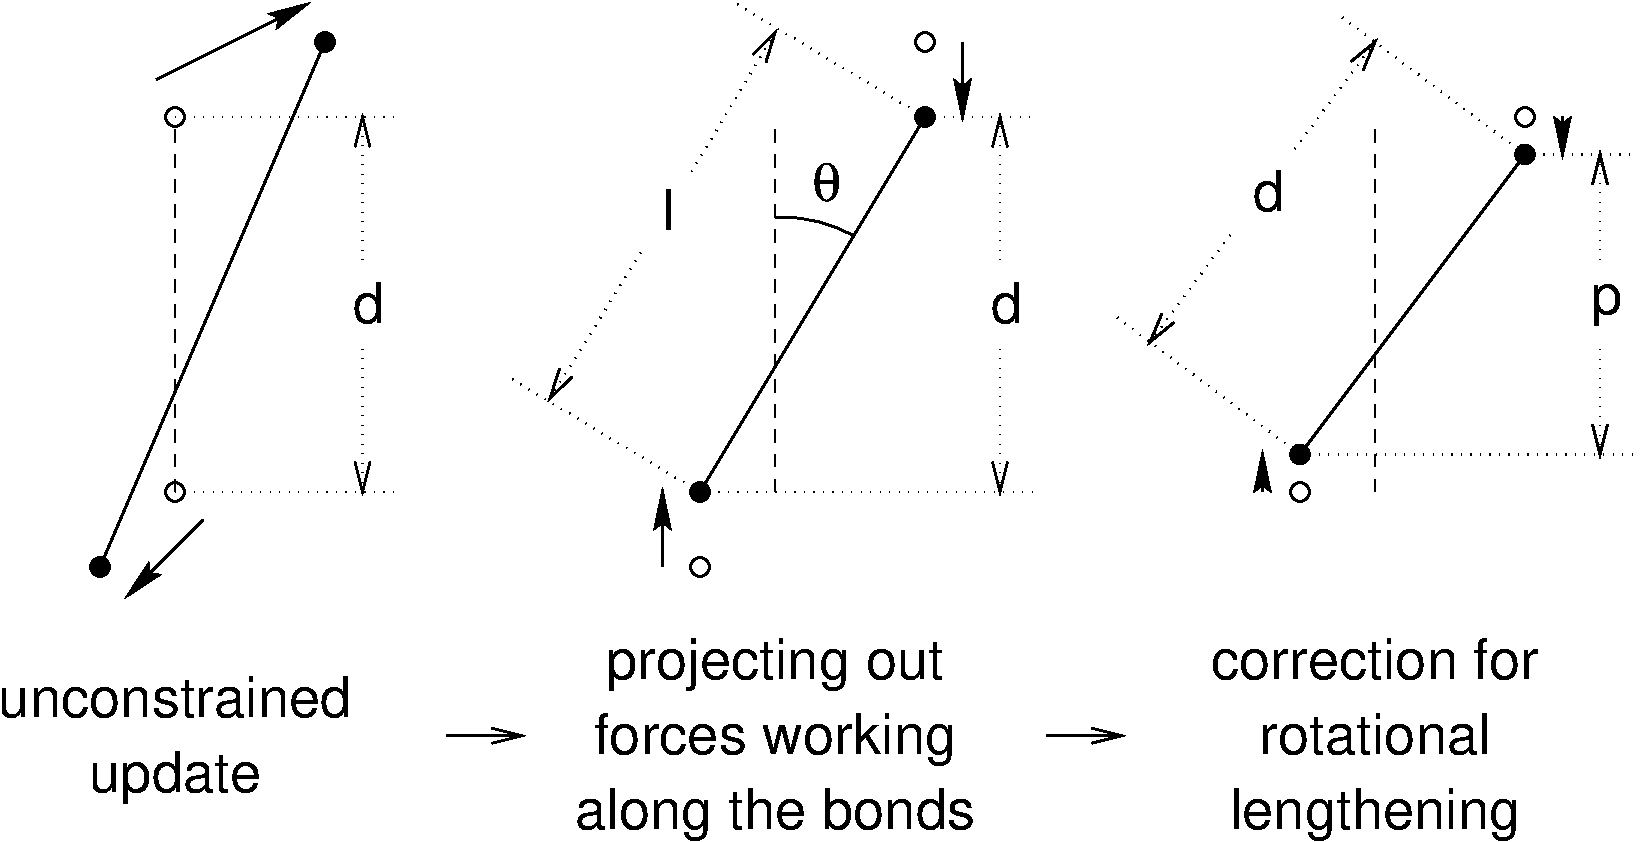
\includegraphics[height=50mm]{plots/lincs}}
\caption[The three position updates needed for one time step.]{The
three position updates needed for one time step. The dashed line is
the old bond of length $d$, the solid lines are the new bonds. $l=d
\cos \theta$ and $p=(2 d^2 - l^2)^{1 \over 2}$.}
\label{fig:lincs}
\end{figure}

A new notation is introduced for the gradient matrix of the constraint 
equations which appears on the right hand side of the equation
\fs{c3}
B_{hi} = {\p g_h \over \p r_i}
\fe
Notice that $\Bm$ is a $K \times 3N$ matrix, it contains the directions
of the constraints.
The following equation shows how the new constrained coordinates 
$\ve{r}_{n+1}$ are related to the unconstrained coordinates
$\ve{r}_{n+1}^{unc}$
\fs{m0}
\begin{array}{c}
  \ve{r}_{n+1}=(\ve{I}-\Tm_n \ve{B}_n) \ve{r}_{n+1}^{unc} + \Tm_n \lenc=  
  \\[2mm]
  \ve{r}_{n+1}^{unc} - 
\iM \Bm_n (\Bm_n \iM \Bm_n^T)^{-1} (\Bm_n \ve{r}_{n+1}^{unc} - \lenc) 
\end{array}
\fe
where $\Tm = \iM \Bm^T (\Bm \iM \Bm^T)^{-1}$.
The derivation of this equation from \eqnsref{c1}{c2} can be found
in \cite{Hess97}.

This first step does not set the real bond lengths to the prescribed lengths,
but the projection of the new bonds onto the old directions of the bonds.
To correct for the rotation of bond $i$, the projection of the
bond on the old direction is set to 
\fs{m1a}
p_i=\sqrt{2 d_i^2 - l_i^2}
\fe
where $l_i$ is the bond length after the first projection.
The corrected positions are 
\fs{m1b}
\ve{r}_{n+1}^*=(\ve{I}-\Tm_n \Bm_n)\ve{r}_{n+1} + \Tm_n \ve{p} 
\fe
This correction for rotational effects is actually an iterative process,
but during MD only one iteration is applied.
The relative constraint deviation after this procedure will be less than
0.0001 for every constraint.
In energy minimization this might not be accurate enough, so the number
of iterations is equal to the order of the expansion (see below).

Half of the CPU time goes to inverting the constraint coupling 
matrix $\Bm_n \iM \Bm_n^T$, which has to be done every time step.
This $K \times K$ matrix
has $1/m_{i_1} + 1/m_{i_2}$ on the diagonal.
The off-diagonal elements are only non-zero when two bonds are connected,
then the element is 
$\cos \phi /m_c$,  where $m_c$ is 
the mass of the atom connecting the
two bonds and $\phi$ is the angle between the bonds.

The matrix $\Tm$ is inverted through a power expansion.
A $K \times K$ matrix $\ve{S}$ is 
introduced which is the inverse square root of 
the diagonal of $\Bm_n \iM \Bm_n^T$.
This matrix is used to convert the diagonal elements 
of the coupling matrix to one
\fs{m2}
\begin{array}{c}
(\Bm_n \iM \Bm_n^T)^{-1}
= \Sm \Sm^{-1} (\Bm_n \iM \Bm_n^T)^{-1} \Sm^{-1} \Sm  \\[2mm]
= \Sm (\Sm \Bm_n \iM \Bm_n^T \Sm)^{-1} \Sm =
  \Sm (\ve{I} - \ve{A}_n)^{-1} \Sm
\end{array}
\fe
The matrix $\ve{A}_n$ is symmetric and sparse and has zeros on the diagonal.
Thus a simple trick can be used to calculate the inverse
\fs{m3}
(\ve{I}-\ve{A}_n)^{-1}= 
        \ve{I} + \ve{A}_n + \ve{A}_n^2 + \ve{A}_n^3 + \ldots
\fe

This inversion method is only valid if the absolute values of all the
eigenvalues of $\ve{A}_n$ are smaller than one.
In molecules with only bond constraints the connectivity is so low
that this will always be true, even if ring structures are present.
Problems can arise in angle-constrained molecules.
By constraining angles with additional distance constraints
multiple small ring structures are introduced.
This gives a high connectivity, leading to large eigenvalues.
Therefore LINCS should NOT be used with coupled angle-constraints.

For molecules with all bonds constrained the eigenvalues of $A$
are around 0.4. This means that with each additional order
in the expansion \eqnref{m3} the deviations decrease by a factor 0.4.
But for relatively isolated triangles of constraints the largest
eigenvalue is around 0.7.
Such triangles can occur when removing hydrogen angle vibrations
with an additional angle constraint in alcohol groups
or when constraining water molecules with LINCS, for instance
with flexible constraints.
The constraints in such triangles converge twice as slow as
the other constraints. Therefore, starting with {\gromacs} 4,
additional terms are added to the expansion for such triangles:
\fs{m3_ang}
(\ve{I}-\ve{A}_n)^{-1} \approx
        \ve{I} + \ve{A}_n + \ldots + \ve{A}_n^{N_i} +
        \left(\ve{A}^*_n + \ldots + {\ve{A}_n^*}^{N_i} \right) \ve{A}_n^{N_i}
\fe
where $N_i$ is the normal order of the expansion and
$\ve{A}^*$ only contains the elements of $\ve{A}$ that couple
constraints within rigid triangles, all other elements are zero.
In this manner the accuracy of angle constraints comes close
to that of the other constraints, while the series of matrix vector
multiplications required for determining the expansion
only needs to be extended for a few constraint couplings.
This procedure is described in the P-LINCS paper\cite{Hess2008a}.

\subsubsection{The LINCS Parameters}
The accuracy of LINCS depends on the number of matrices used
in the expansion \eqnref{m3}. For MD calculations a fourth order
expansion is enough. For Brownian dynamics with
large time steps an eighth order expansion may be necessary.
The order is a parameter in the input file for {\tt mdrun}.
The implementation of LINCS is done in such a way that the 
algorithm will never crash. Even when it is impossible to
to reset the constraints LINCS will generate a conformation
which fulfills the constraints as well as possible.
However, LINCS will generate a warning when in one step a bond 
rotates over more than a predefined angle.
This angle is set by the user in the input file for {\tt mdrun}.

} % Brace matches ifthenelse test for gmxlite


\section{Simulated Annealing}
\label{sec:SA}
The well known \swapindex{simulated}{annealing}
(SA) protocol is supported in {\gromacs}, and you can even couple multiple
groups of atoms separately with an arbitrary number of reference temperatures
that change during the simulation. The annealing is implemented by simply 
changing the current reference temperature for each group in the temperature
coupling, so the actual relaxation and coupling properties depends on the
type of thermostat you use and how hard you are coupling it. Since we are
changing the reference temperature it is important to remember that the system
will NOT instantaneously reach this value - you need to allow for the inherent
relaxation time in the coupling algorithm too. If you are changing the 
annealing reference temperature faster than the temperature relaxation you
will probably end up with a crash when the difference becomes too large.

The annealing protocol is specified as a series of corresponding times and 
reference temperatures for each group, and you can also choose whether you only
want a single sequence (after which the temperature will be coupled to the 
last reference value), or if the annealing should be periodic and restart at 
the first reference point once the sequence is completed. You can mix and
match both types of annealing and non-annealed groups in your simulation.

\newcommand{\vrond}{\stackrel{\circ}{\ve{r}}}
\newcommand{\rond}{\stackrel{\circ}{r}}
\newcommand{\ruis}{\ve{r}^G}

\ifthenelse{\equal{\gmxlite}{1}}{}{
\section{\swapindex{Stochastic}{Dynamics}}
\label{sec:SD}
Stochastic or velocity \swapindex{Langevin}{dynamics} adds a friction
and a noise term to Newton's equations of motion:
\beq
\label{SDeq}
m_i {\de^2 \ve{r}_i \over \de t^2} =
- m_i \xi_i {\de \ve{r}_i \over \de t} + \ve{F}_i(\ve{r}) + \vrond_i
\eeq 
where $\xi_i$ is the friction constant $[1/\mbox{ps}]$ and
$\vrond_i\!\!(t)$  is a noise process with 
$\langle \rond_i\!\!(t) \rond_j\!\!(t+s) \rangle = 
    2 m_i \xi_i k_B T \delta(s) \delta_{ij}$.
When $1/\xi_i$ is large compared to the time scales present in the system,
one could see stochastic dynamics as molecular dynamics with stochastic
temperature-coupling. The advantage compared to MD with Berendsen
temperature-coupling is that in case of SD the generated ensemble is known.
For simulating a system in vacuum there is the additional advantage that there is no
accumulation of errors for the overall translational and rotational
degrees of freedom.
When $1/\xi_i$ is small compared to the time scales present in the system,
the dynamics will be completely different from MD, but the sampling is
still correct.

In {\gromacs} there are two algorithm ot integrate equation (\ref{SDeq}).
An efficient one, where the relative error in the temperature
is $\frac{1}{2}\Delta t\, \xi$.
And a more complex leap frog algorithm~\cite{Gunsteren88},
which has third-order accuracy for any value of $\Delta t\, \xi$.
In this complex algorithm four Gaussian random number are required
per integration step per degree of freedom and with constraints the
coordinates needs to be constrained twice per integration step.
Depending on the computational cost of the force calculation,
this can take a significant part of the simulation time.
Exact continuation of a stochastic dynamics simulation is not possible,
because the state of the random number generator is not stored.
When using SD as a thermostat, an appropriate value for $\xi$ is 0.5 ps$^{-1}$,
since this results in a friction that is lower than the internal friction
of water, while it is high enough to remove excess heat
(unless plain cut-off or reaction-field electrostatics is used).
With this value of $\xi$ the efficient algorithm will usually be accurate
enough.

\section{\swapindex{Brownian}{Dynamics}}
\label{sec:BD}
In the limit of high friction stochastic dynamics reduces to 
Brownian dynamics, also called position Langevin dynamics.
This applies to over-damped systems, 
{\ie} systems in which the inertia effects are negligible.
The equation is:
\beq
{\de \ve{r}_i \over \de t} = \frac{1}{\gamma_i} \ve{F}_i(\ve{r}) + \vrond_i
\eeq 
where $\gamma_i$ is the friction coefficient $[\mbox{amu/ps}]$ and
$\vrond_i\!\!(t)$  is a noise process with 
$\langle \rond_i\!\!(t) \rond_j\!\!(t+s) \rangle = 
    2 \delta(s) \delta_{ij} k_B T / \gamma_i$.
In {\gromacs} the equations are integrated with a simple, explicit scheme:
\beq
\ve{r}_i(t+\Delta t) = \ve{r}_i(t) +
        {\Delta t \over \gamma_i} \ve{F}_i(\ve{r}(t)) 
        + \sqrt{2 k_B T {\Delta t \over \gamma_i}}\, \ruis_i 
\eeq
where $\ruis_i$ is Gaussian distributed noise with $\mu = 0$, $\sigma = 1$.
The friction coefficients $\gamma_i$ can be chosen the same for all
particles or as $\gamma_i = m_i/\xi_i$, where the friction constants
$\xi_i$ can be different for different groups of atoms. 
Because the system is assumed to be over damped, large time-steps
can be used. LINCS should be used for the constraints since SHAKE
will not converge for large atomic displacements.
BD is an option of the {\tt mdrun} program.
} % Brace matches ifthenelse test for gmxlite

\section{Energy Minimization}
\label{sec:EM}
Energy minimization in {\gromacs} can be done using steepest descent,
conjugate gradients, or l-bfgs (limited-memory
Broyden-Fletcher-Goldfarb-Shanno quasi-Newtonian minimizer... we
prefer the abbreviation). EM is just an option of the {\tt mdrun}
program.

\subsection{\normindex{Steepest Descent}}
Although steepest descent is certainly not the most efficient
algorithm for searching, it is robust and easy to implement.

We define the vector $\ve{r}$ as the vector of all $3N$ coordinates.
Initially a maximum displacement $h_0$ ({\eg} 0.01 nm) must be given. 

First the forces $\ve{F}$ and potential energy are calculated.
New positions are calculated by
\beq
\ve{r}_{n+1} =  \ve{r}_n + \frac{\ve{F}_n}{\max (|\ve{F}_n|)} h_n
\eeq
where $h_n$ is the maximum displacement and $\ve{F}_n$ is the force,
or the negative gradient of the  potential $V$. The notation $\max
(|\ve{F}_n|)$ means the largest of the absolute values of the force
components.  The forces and energy are again computed for the new positions \\
If ($V_{n+1} < V_n$) the new positions are accepted and $h_{n+1} = 1.2
h_n$. \\
If ($V_{n+1} \geq V_n$) the new positions are rejected and $h_n = 0.2 h_n$.

The algorithm stops when either a user specified number of force 
evaluations has been performed ({\eg} 100), or when the maximum of the absolute
values of the force (gradient) components is smaller than a specified
value $\epsilon$.
Since force truncation produces some noise in the
energy evaluation, the stopping criterion should not be made too tight
to avoid endless iterations. A reasonable value for $\epsilon$ can be
estimated from the root mean square force $f$ a harmonic oscillator would exhibit at a
temperature $T$ This value is 
\beq
  f = 2 \pi \nu \sqrt{ 2mkT}
\eeq
where $\nu$ is the oscillator frequency, $m$ the (reduced) mass, and
$k$ Boltzmann's constant. For a weak oscillator with a wave number of
100 cm$^{-1}$ and a mass of 10 atomic units, at a temperature of 1 K,
$f=7.7$ kJ~mol$^{-1}$~nm$^{-1}$. A value for $\epsilon$ between 1 and
10 is acceptable.   

\ifthenelse{\equal{\gmxlite}{1}}{}{
\subsection{\normindex{Conjugate Gradient}}
Conjugate gradient is slower than steepest descent in the early stages
of the minimization, but becomes more efficient closer to the energy
minimum.  The parameters and stop criterion are the same as for
steepest descent.  In {\gromacs} conjugate gradient can not be used
with constraints, including the SETTLE algorithm for
water~\cite{Miyamoto92}, as this has not been implemented. If water is
present it must be of a flexible model, which can be specified in the
{\tt mdp} file by
{\tt define = -DFLEXIBLE}\\
This is not really a restriction, since the accuracy of conjugate
gradient is only required for minimization prior to a normal mode
analysis, which can not be performed with constraints.  For most other
purposes steepest descent is efficient enough.
} % Brace matches ifthenelse test for gmxlite

\ifthenelse{\equal{\gmxlite}{1}}{}{
\subsection{\normindex{L-BFGS}}
The original BFGS algorithm works by successively creating better
approximations of the inverse Hessian matrix, and moving the system to
the currently estimated minimum. The memory requirements for this are
proportional to the square of the number of particles, so it is not
practical for large systems like biomolecules. Instead, we use the
L-BFGS algorithm of Nocedal~\cite{Byrd95a,Zhu97a}, which approximates
the inverse Hessian by a fixed number of corrections from previous
steps. This sliding-window technique is almost as efficient as the
original method, but the memory requirements are much lower -
proportional to the number of particles multiplied with the correction
steps. In practice we have found it to converge faster than conjugate
gradients, but due to the correction steps it is not yet parallelized.
It is also noteworthy that switched or shifted interactions usually
improve the convergence, since sharp cut-offs means the potential
function at the current coordinates is slightly different from the
previous steps used to build the inverse Hessian approximation.
} % Brace matches ifthenelse test for gmxlite

\ifthenelse{\equal{\gmxlite}{1}}{}{
\section{Normal Mode Analysis}
\normindex{Normal mode analysis}~\cite{Levitt83,Go83,BBrooks83b} 
can be performed using {\gromacs}, by diagonalization of the mass-weighted
\normindex{Hessian} $H$:
\bea
R^T M^{-1/2} H M^{-1/2} R   &=& \mbox{diag}(\lambda_1,\ldots,\lambda_{3N})
\\
\lambda_i &=& (2 \pi \omega_i)^2
\eea
where $M$ contains the atomic masses, $R$ is a matrix that contains
the eigenvectors as columns, $\lambda_i$ are the eigenvalues
and $\omega_i$ are the corresponding frequencies.

First the Hessian matrix, which is a $3N \times 3N$ matrix where $N$
is the number of atoms, needs to be calculated:
\bea
H_{ij}  &=&     \frac{\partial^2 V}{\partial x_i \partial x_j}
\eea
where $x_i$ and $x_j$ denote the atomic x, y or z coordinates.
In practice, this equation is not used, but the Hessian is
calculated numerically from the force as:
\bea
H_{ij} &=& -
  \frac{f_i({\bf x}+h{\bf e}_j) - f_i({\bf x}-h{\bf e}_j)}{2h}
\\
f_i     &=& - \frac{\partial V}{\partial x_i}
\eea
where ${\bf e}_j$ is the unit vector in direction $j$.
It should be noted that
for a usual Normal Mode calculation, it is necessary to completely minimize 
the energy prior to computation of the Hessian.
What tolerance is required depends on the type of system,
but a rough indication is 0.001 kJ mol$^{-1}$.
This should be done with conjugate gradients or l-bfgs in double precision.

A number of {\gromacs} programs are involved in these
calculations. First the energy should be minimized using {\tt mdrun}.
Then {\tt mdrun} computes the Hessian, note that for generating
the run input file one should use the minimized conformation from
the full precision trajectory file, as the structure file is not
accurate enough.
{\tt \normindex{g\_nmeig}} does the diagonalization and
the sorting of the normal modes according to their frequencies.
Both {\tt mdrun} and {\tt g\_nmeig} should be run in double precision.
The normal modes can be analyzed with the program {\tt g\_anaeig}.
Ensembles of structures at any temperature and for any subset of
normal modes can be generated with {\tt \normindex{g\_nmens}}.
An overview of normal mode analysis and the related principal component
analysis (see \secref{covanal}) can be found in~\cite{Hayward95b}.
} % Brace matches ifthenelse test for gmxlite

\ifthenelse{\equal{\gmxlite}{1}}{}{

\section{Free energy calculations}
\label{sec:fecalc}
\index{free energy calculations}
Free energy calculations can be performed
in {\gromacs} using slow-growth methods. An example problem might be:
calculate the difference in free energy of binding of an inhibitor {\bf I}
to an enzyme {\bf E} and to a mutated enzyme {\bf E$\prime$}.
It is not feasible with computer simulations to perform a docking
calculation for such a large complex, or even releasing the inhibitor from
the enzyme in a reasonable amount of computer time with reasonable accuracy.
However, if we consider the free energy cycle in (\figref{free}A)
we can write
\beq
\Delta G_1 - \Delta G_2 =       \Delta G_3 - \Delta G_4
\label{eqn:ddg}
\eeq
If we are interested in the left-hand term we can equally well compute
the right-hand term.
\begin{figure}
\centerline{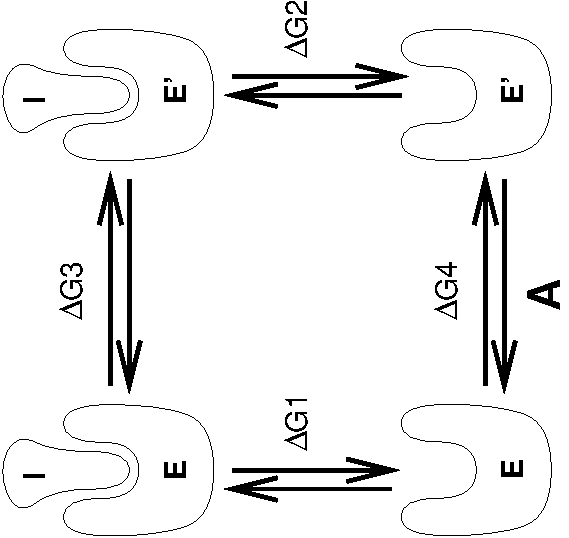
\includegraphics[width=6cm,angle=270]{plots/free1}\hspace{2cm}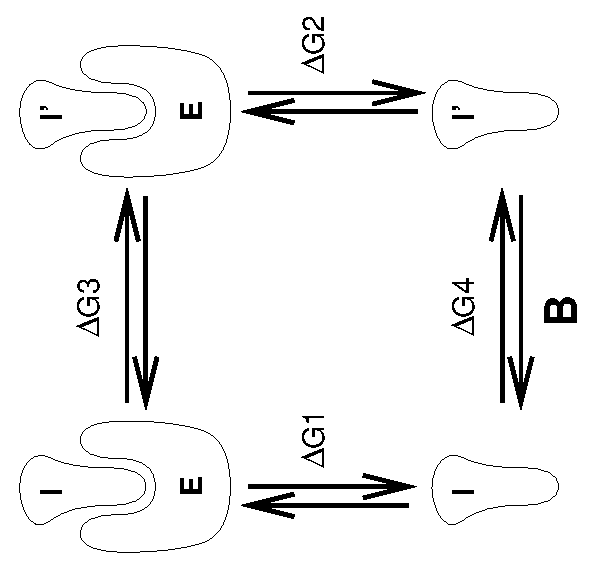
\includegraphics[width=6cm,angle=270]{plots/free2}}
\caption[Free energy cycles.]{Free energy cycles. {\bf A:} to
calculate $\Delta G_{12}$, the free energy difference between the
binding of inhibitor {\bf I} to enzymes {\bf E} respectively {\bf
E$\prime$}. {\bf B:} to calculate $\Delta G_{12}$, the free energy
difference for binding of inhibitors {\bf I} respectively {\bf I$\prime$} to
enzyme {\bf E}.}
\label{fig:free}
\end{figure}

If we want to compute the difference in free energy of binding of two
inhibitors {\bf I} and {\bf I$\prime$} to an enzyme {\bf E} (\figref{free}B)
we can again use \eqnref{ddg} to compute the desired property.

\newcommand{\sA}{^{\mathrm{A}}}
\newcommand{\sB}{^{\mathrm{B}}}
Free energy differences between two molecular species can
be calculated in {\gromacs} using the ``slow-growth'' method. In fact,
such free energy differences between different molecular species are
physically meaningless, but they can be used to obtain meaningful
quantities employing a thermodynamic cycle.
The method requires a simulation during which the Hamiltonian of the
system changes slowly from that describing one system (A) to that
describing the other system (B). The change must be so slow that the
system remains in equilibrium during the process; if that requirement
is fulfilled, the change is reversible and a slow-growth simulation from B to A
will yield the same results (but with a different sign) as a slow-growth
simulation from A to B. This is a useful check, but the user should be
aware of the danger that equality of forward and backward growth results does
not guarantee correctness of the results.

The required modification of the Hamiltonian $H$ is realized by making
$H$ a function of a \textit{coupling parameter} $\lambda:
H=H(p,q;\lambda)$ in such a way that $\lambda=0$ describes system A
and $\lambda=1$ describes system B: 
\beq
  H(p,q;0)=H\sA (p,q);~~~~ H(p,q;1)=H\sB (p,q).
\eeq
In {\gromacs}, the functional form of the $\lambda$-dependence is
different for the various force-field contributions and is described
in section \secref{feia}.

The Helmholtz free energy $A$ is related to the
partition function $Q$ of an $N,V,T$ ensemble, which is assumed to be
the equilibrium ensemble generated by a MD simulation at constant
volume and temperature. The generally more useful Gibbs free energy
$G$ is related to the partition function $\Delta$ of an $N,p,T$
ensemble, which is assumed to be the equilibrium ensemble generated by
a MD simulation at constant pressure and temperature:
\bea
 A(\lambda) &=&  -k_BT \ln Q \\
 Q &=& c \int\!\!\int \exp[-\beta H(p,q;\lambda)]\,dp\,dq \\
 G(\lambda) &=&  -k_BT \ln \Delta \\
 \Delta &=& c \int\!\!\int\!\!\int \exp[-\beta H(p,q;\lambda) -\beta
pV]\,dp\,dq\,dV \\
G &=& A + pV, 
\eea
where $\beta = 1/(k_BT)$ and $c = (N! h^{3N})^{-1}$.
These integrals over phase space cannot be evaluated from a
simulation, but it is possible to evaluate the derivative with 
repect to $\lambda$ as an ensemble average:
\beq
 \frac{dA}{d\lambda} =  \frac{\int\!\!\int (\partial H/ \partial
\lambda) \exp[-\beta H(p,q;\lambda)]\,dp\,dq}{\int\!\!\int \exp[-\beta
H(p,q;\lambda)]\,dp\,dq} = 
\left\langle \frac{\partial H}{\partial \lambda} \right\rangle_{NVT;\lambda},
\eeq
with a similar relation for $dG/d\lambda$ in the $N,p,T$
ensemble.  The difference in free energy between A and B can be found
by integrating the derivative over $\lambda$:
\bea
  A\sB(V,T)-A\sA(V,T) &=& \int_0^1 \left\langle \frac{\partial
H}{\partial \lambda} \right\rangle_{NVT;\lambda} \,d\lambda 
\label{eq:delA} \\
 G\sB(p,T)-G\sA(p,T) &=& \int_0^1 \left\langle \frac{\partial
H}{\partial \lambda} \right\rangle_{NpT;\lambda} \,d\lambda.
\label{eq:delG}
\eea
 
If one wishes to evaluate $G\sB(p,T)-G\sA(p,T)$,
the natural choice is a constant-pressure simulation. However, this
quantity can also be obtained from a slow-growth simulation at
constant volume, starting with system A at pressure $p$ and volume $V$
and ending with system B at pressure $p_B$, by applying the following
small correction: 
\beq
  G\sB(p)-G\sA(p) =
A\sB(V)-A\sA(V) - \int_p^{p\sB}[V\sB(p')-V]\,dp'
\eeq
Here we omitted the constant $T$ from the notation. This correction is
roughly equal to $-\frac{1}{2} (p\sB-p)\Delta V=(\Delta V)^2/(2
\kappa V)$, where $\Delta V$ is the volume change at $p$ and $\kappa$
is the isothermal compressibility. This is usually
negligible. For example, the growth of a water molecule from nothing
in a bath of 1000 water molecules at constant volume would produce an
additional pressure of 22 bar and a correction to the Helmholtz free
energy of -20 J/mol.

In cartesian coordinates, the kinetic energy term in the Hamiltonian
depends only on the momenta, and can be separately integrated and in
fact removed from the equations. When masses do not change, there is
no contribution from the kinetic energy at all; otherwise the
integrated contribution to the free energy is $-\frac{3}{2} k_BT \ln
(m\sB/m\sA)$. This is no longer true in the presence of constraints.
  
{\gromacs} offers the possibility to integrate eq.~\ref{eq:delA} or
eq. \ref{eq:delG} in one simulation over the full range from A to
B. However, if the change is large and sampling insufficiency can be
expected, the user may prefer to determine the value of $\langle
dG/d\lambda \rangle$ accurately at a number of well-chosen
intermediate values of $\lambda$. This can be easily done by setting
the stepsize \textbf{delta\_lambda} to zero. Each simulation can be
equilibrated first, and a proper error estimate can be made for each
value of $dG/d\lambda$ from the fluctuation of $\partial H/\partial
\lambda$. The total free energy change is then determined afterwards
by an appropriate numerical integration procedure.

The $\lambda$-dependence for the force-field contributions is
described in section \secref{feia}.
} % Brace matches ifthenelse test for gmxlite

\ifthenelse{\equal{\gmxlite}{1}}{}{
\section{\normindex{Replica exchange}}
Replica exchange molecular dynamics (\normindex{REMD})
is a method which can be used to speed up
the sampling of any type of simulation, especially if
conformations are separated by relatively high energy barriers.
It involves simulating multiple replicas of the same system
at different temperatures and randomly exchanging the complete state
of two replicas at regular intervals with the probability:
\beq
P(1 \leftrightarrow 2)=\min\left(1,\exp\left[
\left(\frac{1}{k_B T_1} - \frac{1}{k_B T_2}\right)(U_1 - U_2)
 \right] \right)
\eeq
where $T_1$ and $T_2$ are the reference temperatures and $U_1$ and $U_2$
are the instantaneous potential energies of replicas 1 and 2 respectively.
After exchange the velocities are scaled by $(T_1/T_2)^{\pm0.5}$
and a neighbor search is performed the next step.
This combines the fast sampling and frequent barrier-crossing
of the highest temperature with correct Boltzmann sampling at
all the different temperatures~\cite{Hukushima96a,Sugita99}.
We only attempt exchanges for neighboring temperatures as the probability
decreases very rapidly with the temperature difference.
One should not attempt exchanges for all possible pairs in one step.
If, for instance, replicas 1 and 2 would exchange, the chance of
exchange for replicas 2 and 3 not only depends on the energies of
replicas 2 and 3, but also on the energy of replica 1.
In {\gromacs} this is solved by attempting exchange for all 'odd'
pairs on 'odd' attempts and for all 'even' pairs on 'even' attempts.
If we have four replicas: 0, 1, 2 and 3, ordered in temperature
and we attempt exchange every 1000 steps, pairs 0-1 and 2-3
will be tried at steps 1000, 3000 etc. and pair 1-2 at steps 2000, 4000 etc.

How should one choose the temperatures?
The energy difference can be written as:
\beq
U_1 - U_2 =  N_{df} \frac{c}{2} k_B (T_1 - T_2)
\eeq
where $N_{df}$ is the total number of degrees of freedom of one replica
and $c$ is 1 for harmonic potentials and around 2 for protein/water systems.
If $T_2 = (1+\epsilon) T_1$ the probability becomes:
\beq
P(1 \leftrightarrow 2)
  = \exp\left( -\frac{\epsilon^2 c\,N_{df}}{2 (1+\epsilon)} \right)
\approx \exp\left(-\epsilon^2 \frac{c}{2} N_{df} \right)
\eeq
Thus for a probability of $e^{-2}\approx 0.135$
one obtaines $\epsilon \approx 2/\sqrt{c\,N_{df}}$.
With all bonds constrainted one has $N_{df} \approx 2\, N_{atoms}$
and thus for $c$ = 2 one should choose $\epsilon$ as $1/\sqrt{N_{atoms}}$.
However there is one problem when using pressure coupling. The density at
higher temperatures will decrease, leading to higher energy\cite{Seibert2005a}
and this should be taken into account. The {\gromacs} website features a so-called ``REMD'' - calculator, that lets you type in the temperature range and
the number of atoms, and based on that proposes a set of temperatures.

An extension to the REMD for the isobaric-isothermal ensemble was
proposed by Okabe {\em et al.}~\cite{Okabe2001a}. In this work the
exchange probability is modified to:
\beq
P(1 \leftrightarrow 2)=\min\left(1,\exp\left[
\left(\frac{1}{k_B T_1} - \frac{1}{k_B T_2}\right)(U_1 - U_2) +
\left(\frac{P_1}{k_B T_1} - \frac{P_2}{k_B T_2}\right)\left(V_1-V_2\right)
 \right] \right)
\eeq
where $P_1$ and $P_2$ are the respective reference pressures and $V_1$ and
$V_2$ are the respective instantaneous volumes in the simulations.
In most cases the differences in volume are so small that the second
term is negligible. It only plays a role when the difference between
$P_1$ and $P_2$ is large or in phase transitions.

Replica exchange is an option of the {\tt mdrun} program. It will only
work when MPI is installed, due to the inherent parallellism in the
algorithm. For efficiency each replica can run on a separate node.
See the manual page of {\tt mdrun} on how to use it.
} % Brace matches ifthenelse test for gmxlite

\ifthenelse{\equal{\gmxlite}{1}}{}{

\section{\normindex{Essential Dynamics Sampling}}
The results from Essential Dynamics (see \secref{covanal})
of a protein can be used to guide MD simulations. The idea is that
from an initial MD simulation (or from other sources) a definition of
the collective fluctuations with largest amplitude is obtained. The
position along one or more of these collective modes can be
constrained in a (second) MD simulation in a number of ways for
several purposes. For example, the position along a certain mode may
be kept fixed to monitor the average force (free-energy gradient) on
that coordinate in that position. Another application is to enhance
sampling efficiency with respect to usual MD
\cite{Degroot96a,Degroot96b}. In this case, the system is encouraged
to sample its available configuration space more systematically than
in a diffusion-like path that proteins usually take.

Another possiblity to enhance sampling is \normindex{flooding}.
Here a flooding potential is added to certain
(collective) degrees of freedom to expell the system out
of a region of phase space.

The procedure for essential dynamics sampling or flooding is as follows.
First the eigenvectors and eigenvalues need to be determined
using covariance analysis ({\tt g\_covar})
or normal modes analysis ({\tt g\_nmeig}).
This information is fed into {\tt make\_edi}
which has many options for selecting vectors and setting parameters,
see \appref{progman} for the manual page of {\tt make\_edi}.
The generated {\tt edi} input file is then passed to {\tt mdrun}.

} % Brace matches ifthenelse test for gmxlite

% This stuff is quite outdated now.
%\ifthenelse{\equal{\gmxlite}{1}}{}{
%% This file is part of the GROMACS molecular simulation package.
%
% Copyright (c) 2013, by the GROMACS development team, led by
% David van der Spoel, Berk Hess, Erik Lindahl, and including many
% others, as listed in the AUTHORS file in the top-level source
% directory and at http://www.gromacs.org.
%
% GROMACS is free software; you can redistribute it and/or
% modify it under the terms of the GNU Lesser General Public License
% as published by the Free Software Foundation; either version 2.1
% of the License, or (at your option) any later version.
%
% GROMACS is distributed in the hope that it will be useful,
% but WITHOUT ANY WARRANTY; without even the implied warranty of
% MERCHANTABILITY or FITNESS FOR A PARTICULAR PURPOSE. See the GNU
% Lesser General Public License for more details.
%
% You should have received a copy of the GNU Lesser General Public
% License along with GROMACS; if not, see
% http://www.gnu.org/licenses, or write to the Free Software Foundation,
% Inc., 51 Franklin Street, Fifth Floor, Boston, MA  02110-1301  USA.
%
% If you want to redistribute modifications to GROMACS, please
% consider that scientific software is very special. Version
% control is crucial - bugs must be traceable. We will be happy to
% consider code for inclusion in the official distribution, but
% derived work must not be called official GROMACS. Details are found
% in the README & COPYING files - if they are missing, get the
% official version at http://www.gromacs.org.
%
% To help us fund GROMACS development, we humbly ask that you cite
% the research papers on the package. Check out http://www.gromacs.org

\section{Parallelization}
\label{sec:par}

\newcommand{\abs}[1]{\mid \! {#1} \! \mid}

The purpose of this section is to discuss the 
\normindex{parallelization} of the 
principle MD algorithm and not to describe the algorithms that are in 
practical use for molecular systems with their complex variety of atoms 
and terms in the force field descriptions. We shall therefore consider 
as an example a simple system consisting only of a single type of atoms 
with a simple form of the interaction potential. The emphasis will be 
on the special problems that arise when the algorithm is implemented on 
a parallel computer. 

The simple model problem already contains the bottleneck of all MD 
simulations: the computationally intensive evaluation of the 
{\em non-bonded} forces between pairs of atoms, based on the distance 
between particles. Complex molecular systems will in addition 
involve many different kinds of {\em bonded} forces between designated 
atoms. Such interactions add to the complexity of the algorithm but do 
not modify the basic considerations concerning parallelization.


\subsection{Methods of parallelization}
There are a number of methods to parallelize the MD algorithm, each of
them with their own advantages and disadvantages. The method to 
choose depends on the hardware and compilers available.
We list them here:
\begin{enumerate}
\item[1]        {\em \normindex{Message Passing}.}\\
                In this method, which is more or less the traditional
                way of parallel programming, all the parallelism is
                explicitly programmed by the user. The disadvantage
                is that it takes extra code and effort, the advantage
                is that the programmer keeps full control over the data
                flow and can do optimizations a compiler could not come 
                up with. 

                The implementation is typically done by calling a set of 
                library routines to send and receive data to and from 
                other processors. Almost all hardware vendors support 
                this way of
                parallelism in their C and Fortran compilers.
                
\item[2]        {\em \swapindex{Data}{Parallel}.}\\
                This method lets the user define arrays on which to
                operate in parallel. Programming this way is much
                like vectorizing: recurrence is not parallelized
                ({\eg} {\tt for(i=1; (i<MAX); i++) a[i] = a[i-1] + 1;}
                does not vectorize and not parallelize, because for
                every i the result from the previous step is needed).

                The advantage of data parallelism is that it is
                easier for the user; the compiler takes care of the
                parallelism. The disadvantage is that it is supported
                by a small (though growing) number of hardware vendors,
                and that it is much harder to maintain a program that has to
                run on both parallel and sequential machines, because
                the only standard language that supports it is Fortran-90
                which is not available on many platforms.
\end{enumerate}
Both methods allow for the MD algorithm to be implemented without much
trouble. Message passing MD algorithms have been published
since the mid 80's (\cite{Fincham87}, \cite{Raine89}) 
and development is still continuing. 
Data parallel programming is newer,
but starting from a well vectorized program it is not hard to do.

Our implementation of MD is a message passing one, the reason for which
is partly historical: the project to develop a parallel MD program started
when Fortran-90 was still in the making, and no compilers were
expected to be available. 
At current, we still believe that message passing is the way
to go, after having done some experiments with data parallel programming on a
Connection Machine (CM-5), because of portability to other hardware,
the poor performance of the code produced by the compilers 
and because this way of programming
has the same drawback as vectorization: the part of the program that is
not vectorized or parallelized determines the run time of the program
(\normindex{Amdahl's law}).

The approach we took to parallelism was a minimalist one: use as few
non-standard elements in the software as possible, and use the
simplest \swapindex{processor}{topology} that does the job. We therefore 
decided to use a standard language (ANSI-C) with as few non-standard
routines as possible. We only use 5 communication routines that are
non-standard. It is therefore very easy to port our code to other machines.

For an $O(N^2)$ problem like MD, one of the best schemes for the
inter-processor connections is a ring, so our software demands that a
ring is present in the inter-processor connections. A ring can essentially
always be mapped onto another network like a \normindex{hypercube}, a
bus interface (Ethernet {\eg} using 
\seeindex{Message Passing Interface}{MPI} \normindex{MPI}) or 
a \normindex{tree}
(CM-5). Some hardware vendors have very luxurious connection schemes
that connect every processor to every other processor, but we do not
really need it and so do not use it even though it might come in handy
at times. The advantage with this simple scheme is that {\gromacs}
performs extremely well even on inexpensive workstation clusters.

When using a message passing scheme one has to divide the particles 
over processors, which can be done in two ways:
\begin{itemize}
\item   {\em \swapindex{Space}{Decomposition}.}\\
        An element of space is allocated to each processor, when dividing
        a cubic box with edge $b$ over $P$ processors this can be done 
        by giving
        each processor a slab of length $b/P$. This method 
        has the advantage
        that each processor has about the same number of interactions
        to calculate (at least when the simulated system has a homogeneous
        density, like a liquid or a gas). The disadvantage is that a lot of
        bookkeeping is necessary for particles that move over processor
        boundaries. When using more complex systems, such as macromolecules there
        are also 3- and 4-atom interactions that make 
  	the bookkeeping too complicated for our taste.
\item   {\em \swapindex{Particle}{Decomposition}.}\\
        Every processor is allocated a number of particles. When
        dividing $N$ particles over $P$ processors each processor will
        get $N/P$ particles. The implementation of this method
        is described in the next section.
\end{itemize}

\begin {figure}[p]
\centerline{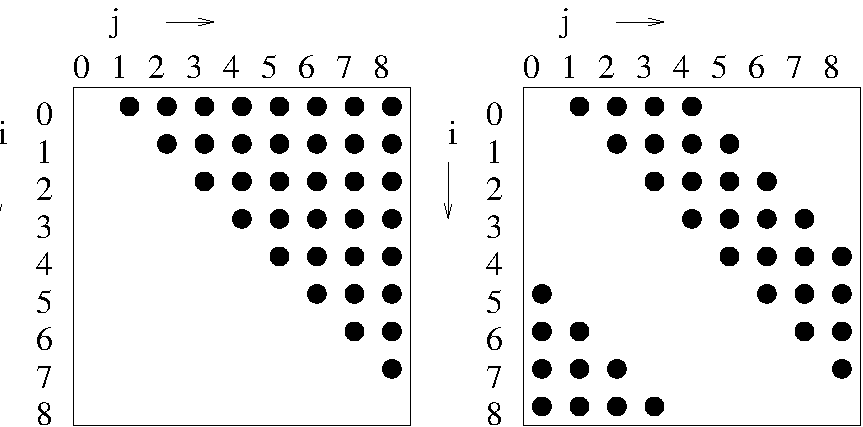
\includegraphics[width=10cm]{plots/int-mat}}
\caption[The interaction matrix.]{The interaction matrix (left) and
the same using action$~=~-$reaction (right).}
\label{fig:int_mat}
\end {figure}

\begin{table}[p]
\centerline{
\newcolumntype{s}[1]{D{/}{/}{#1}}
\begin{tabular}{|l|s4|s4|s4|s4|}
\dline
        & \mcc{1}{i mod 2 = 0}
                & \mcc{1}{i mod 2 = 0}
                                & \mcc{1}{i mod 2 = 1}
                                                & \mcc{1}{i mod 2 = 1} \\
        & \mcc{1}{i $<$ N/2} 
                & \mcc{1}{i $\ge$ N/2}
                                & \mcc{1}{i $<$ N/2}
                                                & \mcc{1}{i $\ge$ N/2} \\
\hline
N mod 2 = 1     & N/2   & N/2           & N/2           & N/2           \\
N mod 4 = 2     & N/2   & N/2           & N/2 - 1       & N/2 - 1       \\
N mod 4 = 0     & N/2   & N/2 - 1       & N/2 - 1       & N/2           \\
\dline
\end{tabular}
}
\caption[The number of interactions between particles.]{The number of
interactions between particles. The number of $j$ particles per $i$
particle is a function of the total number of particles $N$ and
particle number $i$. Note that here the $/$ operator is used for
integer division, {\ie} truncating the reminder.}
\label{tab:decomp}
\end{table}

\begin{figure}[p]
\centerline{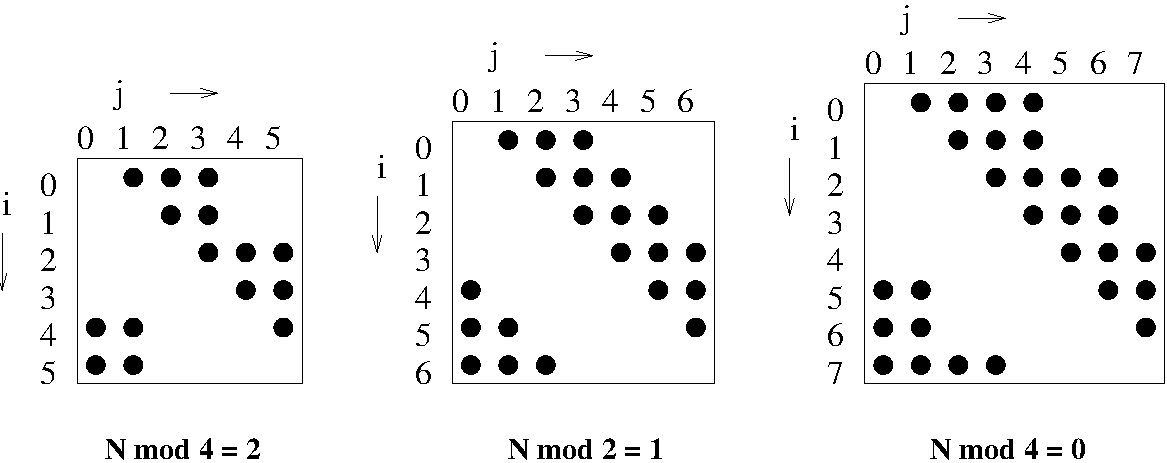
\includegraphics[width=\linewidth]{plots/decomp}}
\caption[Interaction matrices for different $N$.]{Interaction matrices for different $N$. The number of $j$-particles an $i$-particle interacts with depends on the {\em total} number of particles and on the {\em particle number}.}
\label{fig:decomp}
\end{figure}

\subsection{MD on a ring of processors}
When a neighbor list is not used the MD problem is in principle an $O(N^2)$ 
problem as each particle can interact
with every other. This can be simplified using Newton's third law
\beq
F_{ij}  ~=~     -F_{ji}
\label{eqn:Newt3}
\eeq
This implies that there is half a matrix of interactions (without diagonal, 
a particle does not interact with itself) to consider (\figref{int_mat}).
When we reflect the upper right triangle of interactions to the lower
left triangle of the matrix, we still cover all possible interactions,
but now every row in the matrix has almost the same number of points
or possible interactions.  We can now assign a (preferably equal)
number of rows to each processor to compute the forces and at the same
time a number of particles to do the update on, the {\em home}
particles. The number of interactions per particle is dependent on the
{\em total number} $N$ of particles (see \figref{decomp}) and on the
{\em particle number} $i$.  The exact formulae are given in
\tabref{decomp}.

A flow chart of the algorithm is given in \figref{mdpar}.
\begin{figure}
\centerline{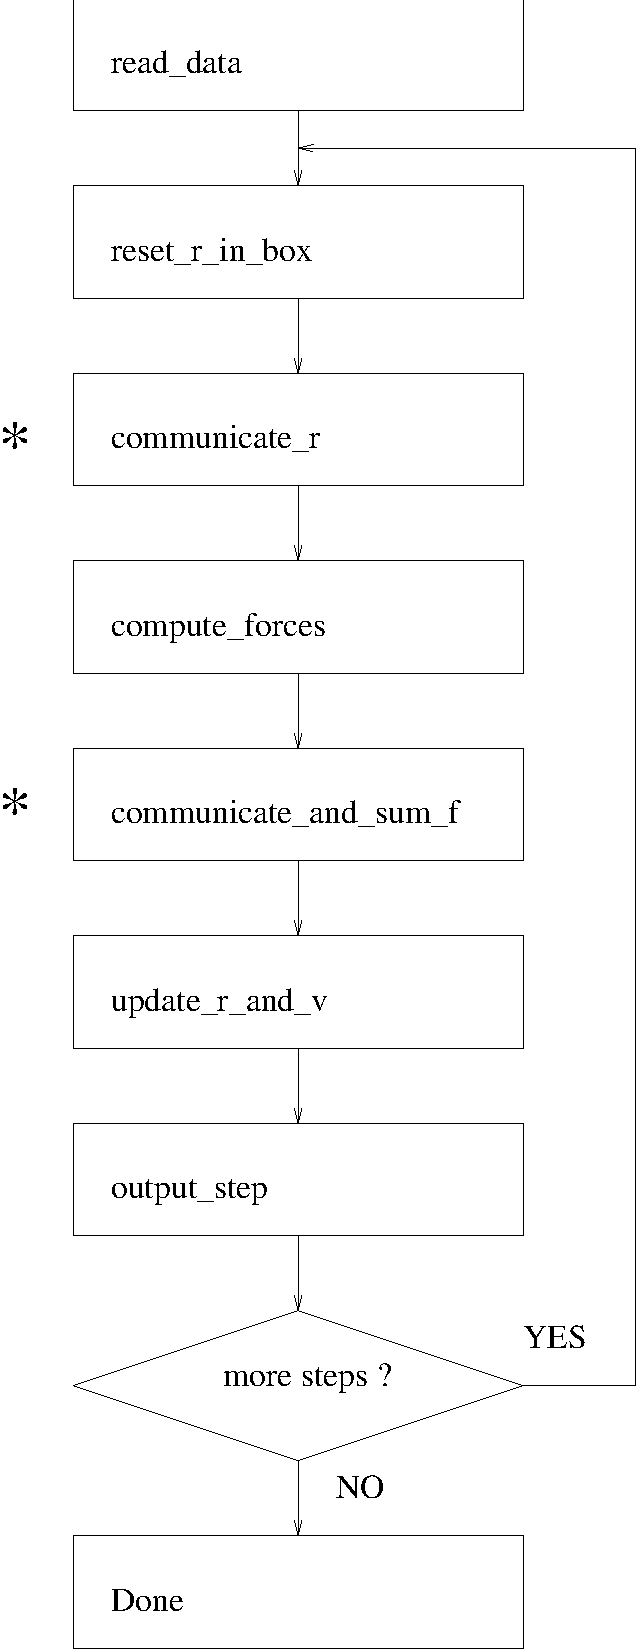
\includegraphics[height=18cm]{plots/mdpar}}
\caption[The Parallel MD algorithm.]{The Parallel MD algorithm. If
the steps marked * are left out we have the sequential algorithm
again.}
\label{fig:mdpar}
\end{figure}
\vfill

It is the same as the sequential algorithm, except for two
communication steps. After the particles have been reset in the box,
each processor sends its coordinates onward (left) and then starts computation
of the forces.  After this step each processor holds the {\em partial
forces} for the available particles, {\eg} processor 0 holds forces
acting on home particles from processor 0, 1, 2 and 3. These forces
must be accumulated and sent back (right) to the home
processor. Finally the update of the velocity and coordinates is done
on the home processor.

The {\tt communicate_r} routine is given below in the full C-code:\\
\begin{footnotesize}
\begin{verbatim}
void communicate_r(int nprocs,int pid,rvec vecs[],int start[],int homenr[])
/* 
 * nprocs = number of processors
 * pid    = processor id (0..nprocs-1)
 * vecs   = vectors
 * start  = starting index in vecs for each processor
 * homenr = number of home particles for each processor
 */
{
  int i;        /* processor counter */
  int shift;    /* the amount of processors to communicate with */
  int cur;      /* current processor to send data from */
  int next;     /* next processor on a ring (using modulo) */

  cur   = pid;
  shift = nprocs/2;

  for (i=0; (i<shift); i++) {
    next=(cur+1) \% nprocs;     
    send   (left,  vecs[start[cur]],  homenr[cur]);
    receive(right, vecs[start[next]], homenr[next]);
    cur=next;
  }
}
\end{verbatim}

\end{footnotesize}

The data flow around the ring is visualized in \figref{ring}. 
Note that because of the ring topology each processor automatically 
gets the proper particles to interact with.
\begin {figure}
\centerline{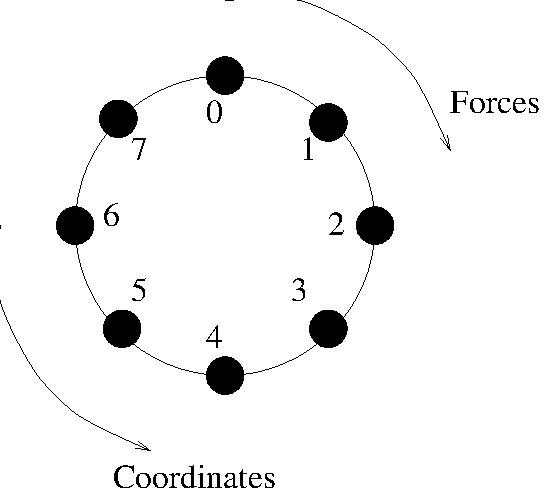
\includegraphics[width=6cm]{plots/ring}}
\caption {Data flow in a ring of processors.}
\label{fig:ring}
\end {figure}

\section{Parallel Molecular Dynamics}
In this chapter we describe some details of the \swapindex{parallel}{MD}  
algorithm used 
in {\gromacs}. This also includes some other information on neighbor searching and
a side excursion to parallel sorting.
Please note the following which we use throughout this chapter:\\
{\bf definition:} {\natom}: Number of particles, {\nproc} number of processors.\\
{\gromacs} employs two different grids: the neighbor searching grid ({\nsgrid})
and the combined charge/potential grid ({\fftgrid}), as will be described below.
To maximize the confusion, 
these two grids are mapped onto a grid of processors when {\gromacs} runs on a 
parallel computer.

\subsection{Domain decomposition}
Modern parallel computers, such as an IBM SP/2 or a Cray T3E
consist of relatively small numbers of relatively fast scalar
processors (typically 8 to 256).  The communication channels that are
available in hardware on these machine are not directly visible to
the programmer; a software layer (usually \normindex{MPI}) 
hides this, and makes communication from all processors to all
others possible. In contrast, in the {\gromacs} hardware~\cite{Berendsen95a}
only communication in a ring was available, {\ie} each processor could communicate
with its direct neighbors only.

It seems logical to map the computational box of an MD simulation system 
to a 3D grid of 
processors ({\eg} 4x4x4 for a 64 processor system). This ensures that most 
interactions that are local in space can be computed with information from 
neighboring processors only. However, this means that there have to be
communication channels in 3 dimensions too, which is not necessarily the case.
Although this may be overcome in software, such a mapping complicates the MD
software as well, without clear performance benefits on most
parallel computers. 

Therefore we opt for a simple one-dimensional division scheme
for the computational box. Each processor gets a slab of this box in the 
X-dimension.
For the communication between processors this has two main advantages:
\begin{enumerate}
\item   Simplicity of coding. Communication can only be to two neighbors
        (called {\em left} and {\em right} in {\gromacs}).
\item   Communication can usually be done in large chunks, which makes it
        more efficient on most hardware platforms.
\end{enumerate}

Most interactions in molecular dynamics have in principle a
short-range character.  Bonds, angles and dihedrals are guaranteed to
have the corresponding particles close in space.


\subsection{Domain decomposition for non-bonded forces}
For large parallel computers, domain decomposition is preferable over
particle decomposition, since it is easier to do load
balancing. Without load balancing the scaling of the code is rather
poor. For this purpose, the computational box is divided in {\nproc}
slabs, where {\nproc} is equal to the number of processors. There are
multiple ways of dividing the box over processors, but since the
{\gromacs} code assumes a ring topology for the processors, it is
logical to cut the system in slabs in just one dimension, the X
dimension.  The algorithm for neighbor searching then becomes:
\begin{enumerate}
\item   Make a list of charge group indices sorted on (increasing) X coordinate
        (\figref{parsort}).
        {\bf Note} that care must be taken to parallelize the sorting algorithm
        as well. See \secref{parsort}.
\item   Divide this list into slabs, with each slab having the same number of
        charge groups
\item   Put the particles corresponding to the local slab on a 3D {\nsgrid} as 
        described in \secref{nsgrid}.
\item   Communicate the {\nsgrid} to neighboring processors (not necessarily to all
        processors). The amount of neighboring {\nsgrid} cells (N$_{gx}$) to 
        communicate is determined by the cut-off length $r_c$ according to
        \beq
        N_{gx}  ~=~     \frac{r_c \nproc}{l_x}   
        \eeq
        where $l_x$ is the box length in the slabbing direction. 
\item   On each processor compute the neighbor list for all charge groups in
        its slab using the normal grid neighbor-searching.
\end{enumerate}

\begin{figure}
\centerline{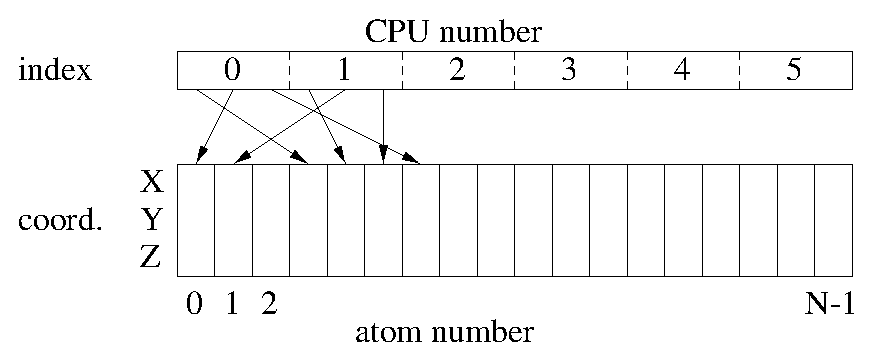
\includegraphics[width=10cm]{plots/parsort}}
\caption[Index in the coordinate array.]{Index in the coordinate
array. The division in slabs is indicated by dashed lines.}
\label{fig:parsort}
\end{figure}

For homogeneous system, this is close to an optimal load balancing,
without actually doing load balancing. For inhomogeneous system, such
as membranes or interfaces, the slabs should be perpendicular to the
interface; this way, each processor has ``a little bit of
everything''.  The {\gromacs} utility program {\tt editconf} has an
option to rotate a whole computational box.

The following observations are important here:
\begin{itemize}
\item   Particles may diffuse from one slab to the other, therefore each processor
        must hold coordinates for all particles all the time, and distribute forces
        back to all processors as well.
\item   Velocities are kept on the ``home processor'' for each particle,
        where the integration of Newton's equations is done.
\item   Fixed interaction lists (bonds, angles etc.) are kept each
        on a single processor.  Since all processors have all
        coordinates, it does not matter where interactions are
        calculated.  The division is actually done by the {\gromacs}
        preprocessor {\tt grompp} and care is taken that, as far as
        possible, every processor gets the same number of bonded
        interactions.
\end{itemize}

In all, this makes for a mixed particle decomposition/domain decomposition scheme
for parallelization of the MD code. The communication costs are four times higher
than for the simple particle decomposition method described in \secref{par}
(the whole coordinate and force array are communicated across the whole ring,
rather than half the array over half the ring).
However, for large numbers of processors the improved load balancing 
compensates this easily.

\subsection{Parallel \normindex{PPPM}}
A further reason for domain decomposition is the PPPM algorithm. This
algorithm works with a 3D Fast Fourier Transform. It employs a
discrete grid of dimensions (\nx,\ny,\nz), the {\fftgrid}. The
algorithm consist of five steps, each of which have to be
parallelized:
\begin{enumerate}
\item   Spreading charges on the {\fftgrid} to obtain the charge 
        distribution $\rho(\ve{r})$.
        This bit involves the following sub-steps:
        \begin{enumerate}
        \item[{\bf a.}] put particle in the box
        \item[{\bf b.}] find the {\fftgrid} cell in which the particle resides
        \item[{\bf c.}] add the charge of the particle times the appropriate
                        weight factor (see \secref{pppm}) to 
                        each of the 27 grid points (3 x 3 x 3).
        \end{enumerate}
        In the parallel case, the {\fftgrid} 
        must be filled on each processor with its
        share of the particles, and subsequently the {\fftgrid}s of all processors
        must be summed to find the total charge distribution. It may be clear that
        this induces a large amount of unnecessary work, unless we use domain
        decomposition. If each processor only has particles in a certain region
        of space, it only has to calculate the charge distribution for 
        that region of space. Since {\gromacs} works with slabs, this means that
        each processor fills the {\fftgrid} cells corresponding to its slab in space
        and addition of {\fftgrid}s need only be done for neighboring slabs.\\
        To be more precise, the slab $x$ for processor $i$ is defined as:
        \beq
        i\, \frac{l_x}{M} \le x <\, (i+1)\frac{l_x}{M}
        \eeq
        Particle with this $x$ coordinate range will add to the charge distribution
        on the following range of 
        of {\fftgrid} slabs in the $x$ direction:
        \beq
        {\rm trunc}\left(i\,\frac{l_x \nx}{M}\right)-1 \le i_x \le {\rm trunc}\left((i+1)\,\frac{l_x \nx}{M}\right)+2
        \eeq
        where trunc indicates the truncation of a real number to the largest integer
        smaller than or equal to that real number.
        
\item   Doing the Fourier transform of the charge distribution $\rho(\ve{r})$ 
        in parallel to obtain $\hat{\rho}(\ve{k})$. This is done using
        the FFTW library (see \href{http://www.fftw.org}{www.fftw.org})
        which employs the MPI library for message passing programs
        (note that there are also \swapindex{shared}{memory} versions
        of the FFTW code).\\
        This FFT algorithm actually use slabs as well (good
        thinking!).  Each processor does 2D FFTs on its slab, and then
        the whole {\fftgrid} is transposed {\em in place}
        ({\ie} without using extra memory).  This means that after the
        FFT the X and Y components are swapped.  To complete the FFT,
        this swapping should be undone in principle (by transposing
        back).  Happily the FFTW code has an option to omit this,
        which we use in the next step.
\item   Convolute $\hat{\rho}(\ve{k})$ with the Fourier transform of the
        charge spread function $\hat{g}(\ve{k})$ (which we have tabulated before)
        to obtain the potential $\hat{\phi}(k)$. 
        As an optimization, we store the $\hat{g}(\ve{k})$  in transposed form
        as well, matching the transposed form of $\hat{\rho}(\ve{k})$
        which we get from the FFTW routine. After this step we have the 
        potential $\hat{\phi}(k)$ in Fourier space, but still on the transposed
        {\fftgrid}.
\item   Do an inverse transform of $\hat{\phi}(k)$ to obtain
        ${\phi}(\ve{r})$. Since the algorithm must do a transpose of the data
        this step actually yields the wanted result: the un-transposed
        potential in real space.
\item   Interpolate the potential ${\phi}(\ve{r})$ in real space at the particle
        positions to obtain forces and energy. For this bit the same considerations
 	about parallelism hold as for the charge spreading. However in this
        case more neighboring grid cells are needed, implying that we need
        the following set of {\fftgrid} slabs in the $x$ direction:
        \beq
        {\rm trunc}\left(i\,\frac{l_x \nx}{M}\right)-3 \le i_x \le {\rm trunc}\left((i+1)\,\frac{l_x \nx}{M}\right)+4
        \eeq

\end{enumerate}
The algorithm as sketched above requires communication for spreading
the charges, for the forward and backward FFTs, and for interpolating
the forces.  The {\gromacs} bits of the program use only left and
right communication, {\ie} using two communication channels. The FFTW
routines actually use other forms of communication as well, and these
routines are coded with MPI routines for message passing. This implies
that {\gromacs} can only perform the PPPM algorithm on parallel
computers that support MPI. However, most
\swapindex{shared}{memory} computers, such as the SGI Origin, also
support MPI using the 
shared memory for communication.

\subsection{Parallel sorting}
\label{sec:parsort}
For the domain decomposition bit of {\gromacs} it is necessary to sort the 
coordinates (or rather the index to coordinates) every time a neighbor list is made.
If we use brute force, and sort all coordinates on each processor (which is 
technically possible since we have all the coordinates), then this sorting procedure
will take a constant wall clock time, proportional to {\natom}$^2\log${\natom}, 
regardless of the number of processors. We can however do a little
better, if we assume that particles diffuse only slowly.
A parallel sorting algorithm can be conceived as follows: \\
At the first step of the simulation
\begin{enumerate}
\item   Do a full sort of all indices using {\eg} the  Quicksort algorithm that is
        built-in in the standard C-library
\item   Divide the sorted array into slabs (as described above see 
        \figref{parsort}).
\end{enumerate}
At subsequent steps of the simulation:
\begin{enumerate}
\item   Send the indices for each processor to the preceding processor (if
        not processor 0) and to the next processor (if not {\nproc}-1). The 
        communication associated with this operation is proportional to
        2{\natom}/{\nproc}.
\item   Sort the combined indices of the three (or two) processors. Note that
        the CPU time associated with sorting is now
        (3{\natom}/{\nproc})$^2\log$ (3{\natom}/{\nproc}).
\item   On each processor, the indices belonging to its slab can be determined
        from the order of the array (\figref{parsort}).
\end{enumerate}

%\section{A Worked Example}
%Suppose our box size is 4.0 nm and the cut-off is 0.8 nm. For neighborsearching 
%we use {\dgrid} = 2, such that there 10 {\nsgrid} cells.


% LocalWords:  Parallelization parallelization parallelize Fortran vectorizing
% LocalWords:  parallelized vectorize Amdahl's MPI ij ji decomp mdpar nprocs gx
% LocalWords:  pid rvec vecs homenr dihedrals indices parsort nsgrid editconf
% LocalWords:  preprocessor grompp PPPM pppm trunc FFTW FFT FFTs Convolute un
% LocalWords:  SGI Quicksort formulae

%} % Brace matches ifthenelse test for gmxlite

\section{\normindex{Parallelization}}
The CPU time required for a simulation can be reduced by running the simulation
in parallel over more than one processor or processor core.
Ideally one would want to have linear scaling: running on $N$ processors/cores
makes the simulation $N$ times faster. In practice this can only be
achieved for a small number of processors. The scaling will depend
a lot on the algorithms used. Also different algorithms can have different
restrictions on the interaction ranges between atoms.
In {\gromacs} we have two types of parallelization: particle decomposition
and domain decomposition. Particle decomposition is only useful for
a few special cases. Domain decomposition, which is the default algorithm,
will always be faster and scale better.

\section{\swapindex{Particle}{decomposition}}
Particle decomposition, also called \swapindex{force}{decomposition},
is the simplest type of decomposition. Here at the start of the simulation
particles are assigned to processors. Then forces between particles
need to be assigned to processors such that the force load is evenly balanced.
This decomposition requires that each processor knows the coordinates
of at least half of the particles in the system.
Thus for a high number of processors $N$, about $N \times N/2$ coordinates
need to be communicated. Because of this quadratic relation
particle decomposition does not scale well.

Particle decomposition was the only method available before version 4
of {\gromacs}. Now it is only useful in cases where domain decomposition
does not work. This is for systems with long-range bonded interactions,
especially NMR distance or orientation restraints.
With particle decomposition only whole molecules can be assigned to a processor.

\section{\swapindex{Domain}{decomposition}}
Since most interactions in molecular simulations are local,
domain decomposition is a natural way to decompose the system.
In domain decomposition a spatial domain is assigned to each processor.
Each processor will integrate the equations of motion for the particles
that currently reside in its local domain. With domain decomposition
there are two choices that have to be made: the division of the unit cell
in domains and the assignment of the forces to processors.
Most molecular simulation packages use the half-shell method for assigning
the forces. But there are two methods which always require less communication:
the eighth shell\cite{Liem1991} and the midpoint\cite{Shaw2006} method.
{\gromacs} currently uses the eighth shell method, but for certain systems
or hardware architectures it might be advantageous to use the midpoint
method. Therefore we might implement the midpoint method in the future.
Most of the details of the domain decomposition can be found
in the {\gromacs} 4 paper\cite{Hess2008b}.

\subsection{Coordinate and force communication}
In the most general case of a triclinic unit cell,
the space in divided with a 1, 2 or 3-D grid in parallelepipeds
which we call domain decomposition cells.
Each cell is assigned to a processor.
The system is partitioned over the processors at the beginning
of each MD step where neighbor searching is performed.
Since the neighbor searching is based on charge groups, charge groups
are also the units for the domain decomposition.
Charge groups are assigned to the cell where their center of geometry resides.
Before the forces can be calculated, the coordinates from some
neighboring cells need to be communicated
and after the forces are calculated the forces need to be communicated
in the other direction.
The communication and force assignment is based on zones which
can cover one or multiple cells.
An example of a zone setup is shown in \figref{ddcells}.

\begin{figure}
\centerline{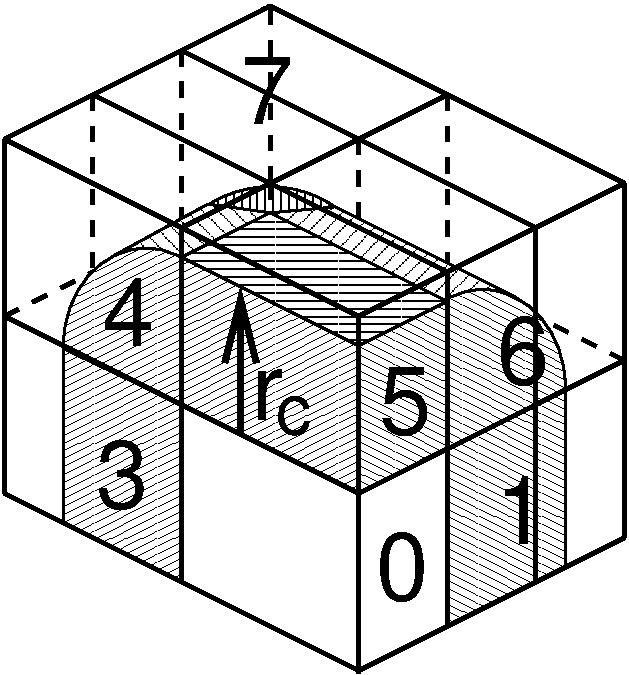
\includegraphics[width=6cm]{plots/dd_cells}}
\caption{
A non-staggered domain decomposition grid of 3$\times$2$\times$2 cells.
Coordinates in zones 1 to 7 are communicated to the corner cell
that has its home particles in zone 0.
$r_c$ is the cut-off radius. 
\label{fig:ddcells}
}
\end{figure}

The coordinates are communicated by moving data along the ``negative''
direction in $x$, $y$ or $z$ to the next neighbor. This can be done in one
or multiple pulses. In \figref{ddcells} two pulses in $x$ are required,
then one in $y$ and then one in $z$. The forces are communicated by
reversing this procedure. See the {\gromacs} 4 paper\cite{Hess2008b}
for details on determining which non-bonded and bonded forces
should be calculated on which node.

\subsection{Dynamic load balancing}
When different processors have a different computational load
(load imbalance), all processors will have to wait for the one
that takes the most time. One would like to avoid such a situation.
Load imbalance can occur due to three reasons:
\begin{itemize}
\item inhomogeneous particle distribution
\item inhomogeneous interaction cost distribution (charged/uncharged,
  water/non-water due to {\gromacs} water innerloops)
\item statistical fluctuation (only with small particle numbers)
\end{itemize}
So we need a dynamic load balancing algorithm
where the volume of each domain decomposition cell
can be adjusted {\em independently}.
To achieve this the 2 or 3-D domain decomposition grids need to be
staggered. \figref{ddtric} shows the most general case in 2-D.
Due to the staggering one might require two distance checks
for deciding if a charge group needs to be communicated:
a non-bonded distance and a bonded distance check.

\begin{figure}
\centerline{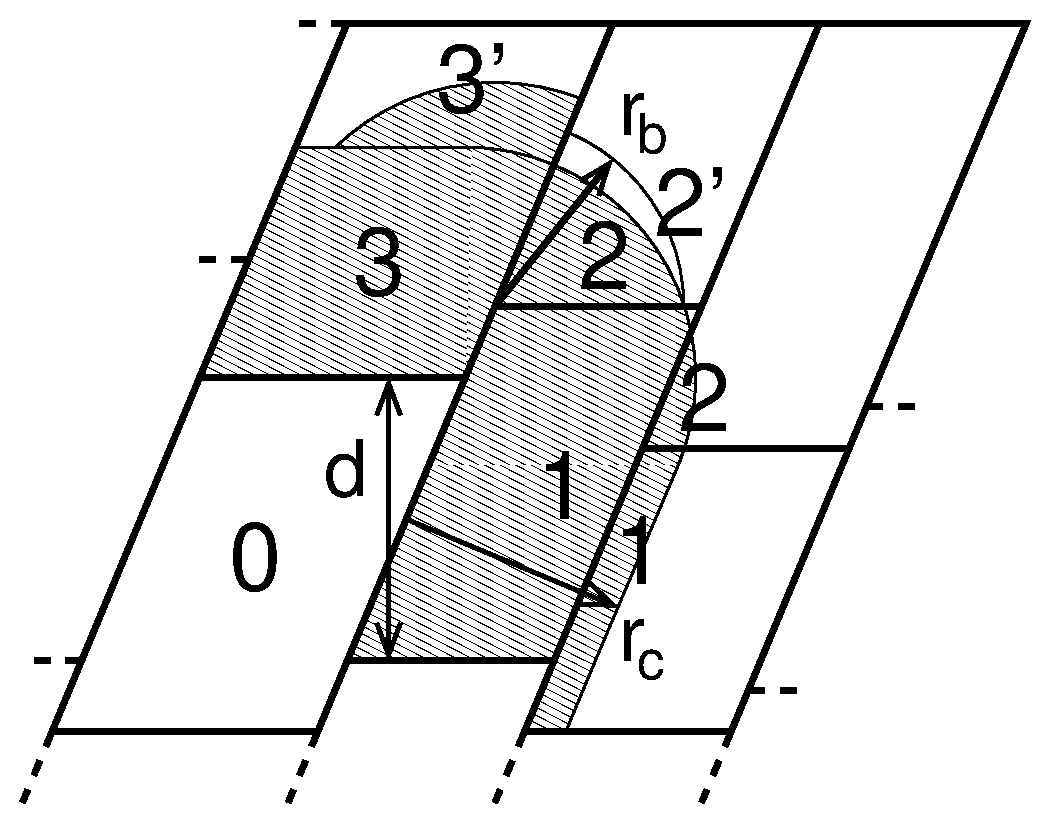
\includegraphics[width=7cm]{plots/dd_tric}}
\caption{
The zones to communicate to the processor of zone 0,
see the text for details. $r_c$ and $r_b$ are the non-bonded
and bonded cut-off radii respectively, $d$ is an example
of a distance between following, staggered boundaries of cells.
\label{fig:ddtric}
}
\end{figure}

By default {\tt mdrun} automatically turns on the dynamic load
balancing during a simulation when the total performance loss
due to the force calculation imbalance is 5\% or more.
Note that the reported force load imbalance numbers might be higher,
since the force calculation is only part of work that needs to be done
during an integration step.
The load imbalance is reported in the log file at log output steps
and when the {\tt -v} option is used also on screen.
The average load imbalance and the total performance loss
due to load imbalance are reported at the end of the log file.

There is one important parameter for the dynamic load balancing
which is the minimum allowed scaling. By default each dimension
of the domain decomposition cell can scale down by at least
a factor of 0.8. For 3-D domain decomposition this allows cells
to change their volume by about a factor of 0.5, which should allow
for compensation of a load imbalance of 100\%.
The required scaling can be changed with the {\tt -dds} option of {\tt mdrun}.

\subsection{Constraints in parallel}
\label{subsec:plincs}
Since with domain decomposition parts of molecules can reside
on different processors, bond constraints can cross cell boundaries.
Therefore a parallel constraint algorithm is required.
{\gromacs} uses the \normindex{P-LINCS} algorithm\cite{Hess2008a},
which is the parallel version of the \normindex{LINCS} algorithm\cite{Hess97}
(see \ssecref{lincs}).
The P-LINCS procedure is illustrated in \figref{plincs}.
When molecules cross the cell boundaries, atoms in such molecules
up to LINCS order plus one bonds away are communicated over the cell boundaries.
Then the normal LINCS algorithm can be applied to the local bonds
plus the communicated ones. After this procedure the local bonds
are correctly constrained, even though the extra communicated ones are not.
One coordinate communication step is required for the initial LINCS step
and one for each iteration. Forces do not need to be communicated.

\begin{figure}
\centerline{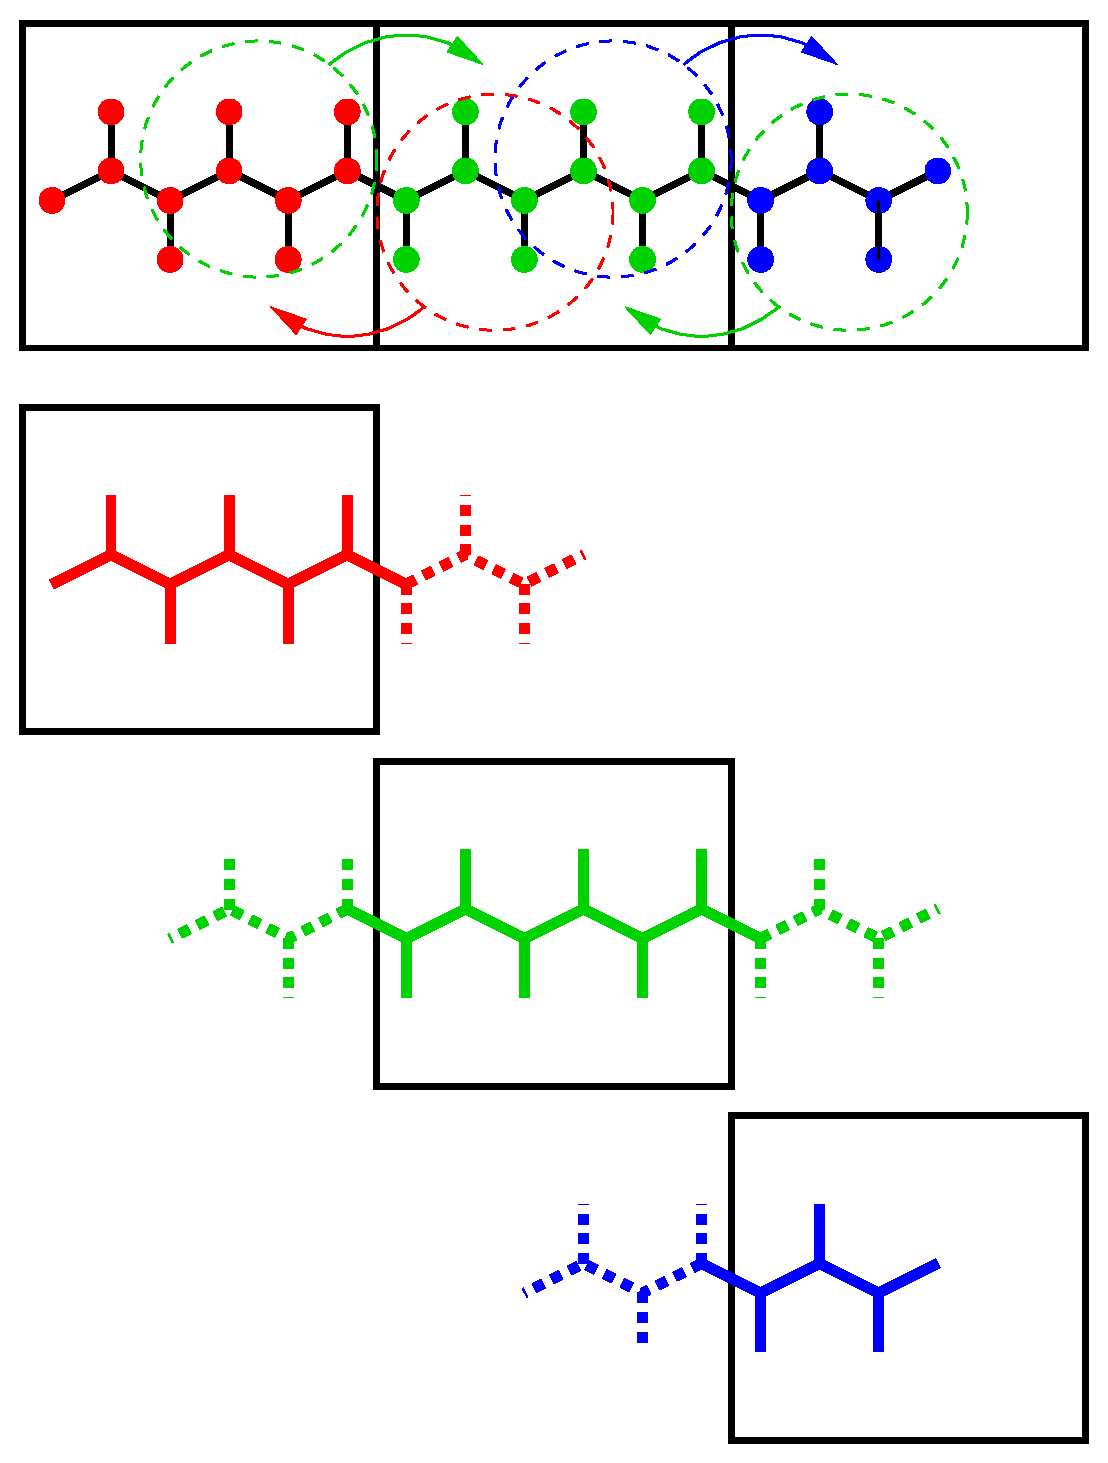
\includegraphics[width=6cm]{plots/par_lincs2}}
\caption{
Example of the parallel setup of P-LINCS with one molecule
split over three domain decomposition cells, using a matrix
expansion order of 3.
The top part shows which atom coordinates need to be communicated
to which cells. The bottom parts show the local constraints (solid)
and the non-local constraints (dashed) for each of the three cells.
\label{fig:plincs}
}
\end{figure}

\subsection{Interaction ranges}
Domain decomposition takes advantage of the locality of interactions.
This means that there will be limitations on the range of interactions.
By default {\tt mdrun} tries to find the optimal balance between
interaction range and efficiency. But it can happen that a simulation
stops with an error message about missing interactions,
or that a simulation might run slightly faster with shorter
interaction ranges. A list of interaction ranges
and their default values is given in \tabref{dd_ranges}.

\begin{table}
\centerline{
\begin{tabular}{|c|c|ll|}
\dline
interaction & range & option & default \\
\dline
non-bonded        & $r_c$ = max($r_{list}$,$r_{VdW}$,$r_{Coul}$) & {\tt mdp} file & \\
two-body bonded   & max($r_{mb}$,$r_c$) & {\tt mdrun -rdd} & starting conf. + 10\% \\
multi-body bonded & $r_{mb}$ & {\tt mdrun -rdd} & starting conf. + 10\% \\
constraints       & $r_{con}$ & {\tt mdrun -rcon} & est. from bond lengths \\
virtual sites     & $r_{con}$ & {\tt mdrun -rcon} & 0 \\
\dline
\end{tabular}
}
\caption{The interaction ranges with domain decomposition.}
\label{tab:dd_ranges}
\end{table}

In most cases the defaults of {\tt mdrun} should not cause the simulation
to stop with an error message of missing interactions.
The range for the bonded interactions is determined from the distance
between bonded charge-groups in the starting configuration, 10\% is added
for headroom. For the constraints the $r_{con}$ is determined by
taking the maximum distance that LINCS order plus one bonds can cover
when they all connect at angles of 120 degrees.
The actual constraint communication is not limited by $r_{con}$,
but by the minimum cell size $L_C$, which has the following lower limit:
\beq
L_C \geq \max(r_{mb},r_{con})
\eeq
Without domain decomposition the system is actually allowed to scale
beyond this limit when pressure scaling is used.
Note that for triclinic boxes $L_C$ is not simply the box diagonal
component divided by the number of cells in that direction,
but it is the shortest distance between the triclinic cells borders.
For rhombic dodecahedra this is a factor of $1/\sqrt{2}$ shorter
along $x$ and $y$.

When $r_{mb} > r_c$, {\tt mdrun} employs a smart algorithm to reduce
the communication. Simply communicating all charge groups within
$r_{mb}$ would increase the amount of communication enormously.
Therefore only charge-groups that are connected by bonded interactions
to charge groups which are not locally present are communicated.
This leads to little extra communication, but also to a slightly
increased cost for the domain decomposition setup.
In some cases, e.g. coarse-grained simulations with a very short cut-off,
one might want to set $r_{mb}$ by hand to reduce this cost.

\subsection{Multiple-Program, Multiple-Data PME parallelization}
\label{subsec:mpmd_pme}
Electrostatics interactions are long range, therefore special
algorithms are used to avoid summation over many atom pairs.
In {\gromacs} this is usually PME (\secref{pme}).
Since with PME all particles interact with each other, global communication
is required. This will usually be the limiting factor on
the scaling with domain decomposition.
To reduce the effect of this problem, we have come up with
a Multiple-Program, Multiple-Data approach\cite{Hess2008b}.
Here some processors are selected to do only the PME mesh calculation,
while the other processors, called particle-particle (PP) nodes,
do all the rest of the work.
For rectangular boxes the optimal PP to PME node ratio is usually 3:1,
for rhombic dodecahedra usually 2:1.
When the number of PME nodes is reduced by a factor of 4, the number
of communication calls is reduced by about a factor of 16.
Or put differently, we can now scale to 4 times more nodes.
In addition, for modern 4 or 8 core machines in a network
the effective network bandwidth for PME is quadrupled,
since only a quarter of the cores will be using the network connection
on each machine during the PME calculations.

\begin{figure}
\centerline{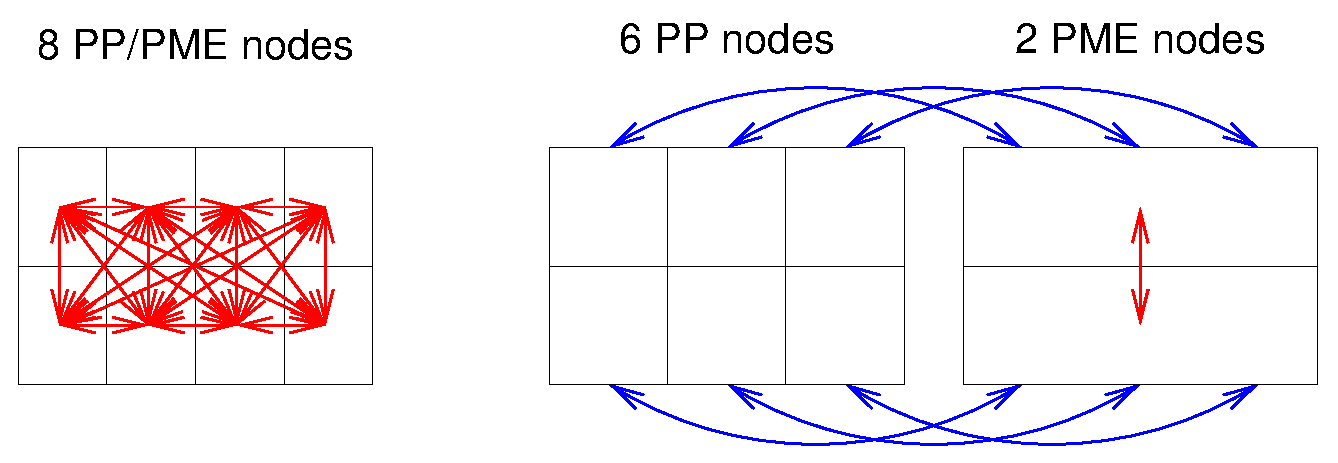
\includegraphics[width=12cm]{plots/mpmd_pme}}
\caption{
Example of 8 nodes without (left) and with (right) MPMD.
The PME communication (red arrows) is much higher on the left
than on the right. For MPMD additional PP - PME coordinate
and force communication (blue arrows) is required,
but the total communication complexity is lower.
\label{fig:mpmd_pme}
}
\end{figure}

{\tt mdrun} will by default interleave the PP and PME nodes.
If the processors are not number consecutively inside the machines,
one might want to use {\tt mdrun -ddorder pp\_pme}.
For machines with a real 3-D torus and proper communication software
that assigns the processors accordingly one should use
{\tt mdrun -ddorder cartesian}.

To optimize the performance one should usually set up the cut-off's
and the PME grid such that the PME load is 25 to 33\% of the total
calculation load. {\tt grompp} will print an estimate for this load
at the end and also {\tt mdrun} calculates the same estimate
to determine the optimal number of PME nodes to use.
For high parallelization it might be worth to optimize
the PME load with the {\tt mdp} settings and/or the number
of PME nodes with the {\tt -npme} option of {\tt mdrun}.
For changing the electrostatics settings it is useful to know
the accuracy of the electrostatics remains nearly constant
when the Coulomb cut-off and the PME grid spacing are scaled
by the same factor.
Note that it is usually better to overestimate than to underestimate
the number of PME nodes, since the number of PME nodes is smaller
than the number of PP nodes, which leads to less total waiting time.

Currently the PME domain decomposition is 1-D along the $x$ axis.
To avoid superfluous communication of coordinates and forces
between the PP and PME nodes, the number of DD cells in the $x$
direction should ideally be the same or a multiple of the number
of PME nodes. By default {\tt mdrun} takes care of this issue.
In the future we will support better parallelizable electrostatics
implementations.

\subsection{Domain decomposition flow chart}
In \figref{dd_flow} a flow chart is shown for domain decomposition
with all possible communication for different algorithms.
For simpler simulations the same flow chart applies,
but simply without the algorithms and communication for
the algorithms which are not used.

\begin{figure}
\centerline{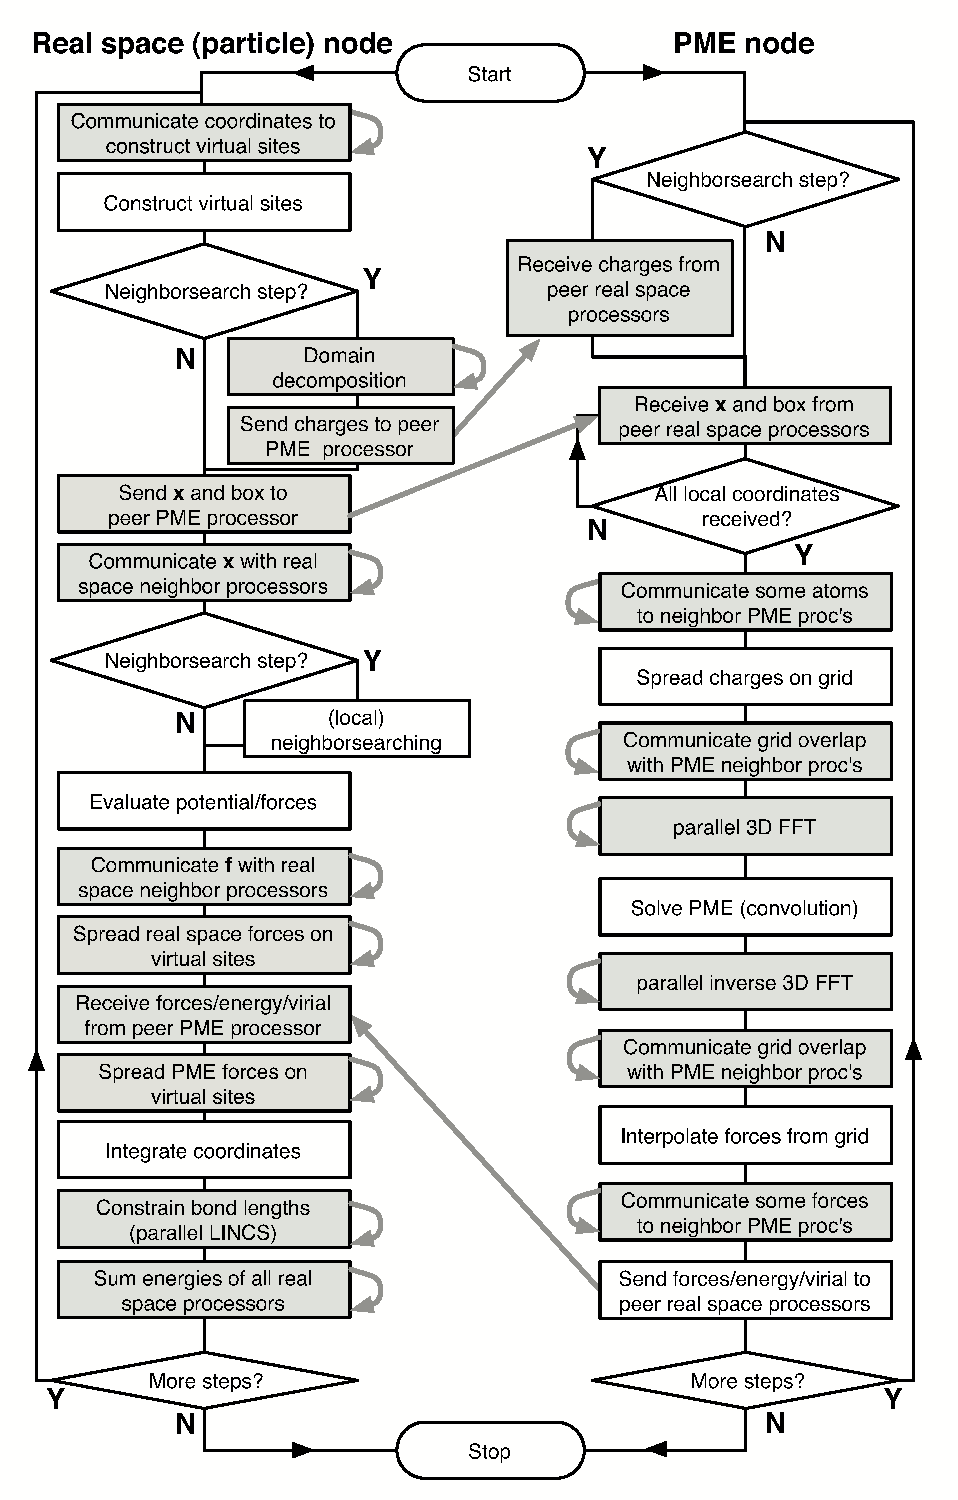
\includegraphics[width=12cm]{plots/flowchart}}
\caption{
Flow chart showing the algorithms and communication (arrows)
for a standard MD simulation with virtual sites, constraints
and separate PME-mesh nodes.
\label{fig:dd_flow}
}
\end{figure}
